\documentclass[11pt,a4paper]{article}
\usepackage{fontspec}
\ifdefined\ReportFontPath
\setmainfont[Path=\ReportFontPath,BoldFont=NotoSerifCJKsc-Regular.otf,BoldFeatures={FakeBold=1.5},ItalicFont=NotoSerifCJKsc-Regular.otf,ItalicFeatures={FakeSlant=.14}]{NotoSerifCJKsc-Regular.otf}
\setmonofont[Path=\ReportFontPath,Scale=.9]{NotoSerifCJKsc-Regular.otf}
\else
\setmainfont[BoldFont={Noto Serif CJK SC Bold},ItalicFeatures={FakeSlant=.14}]{Noto Serif CJK SC}
\setmonofont[Scale=.9]{Noto Serif CJK SC}
\fi
\XeTeXlinebreaklocale "zh"
\XeTeXlinebreakskip=0pt plus 1pt
\usepackage[a4paper,margin=22mm,headheight=16pt]{geometry}
\usepackage{amsmath,amssymb,amsthm,mathtools,bm}
\usepackage{graphicx,booktabs,longtable,tabularx,array,enumitem}
\usepackage{needspace}
\usepackage{xcolor,hyperref,fancyhdr,tcolorbox}
\usepackage{tikz}
\usetikzlibrary{arrows.meta,positioning}
\hypersetup{colorlinks=true,linkcolor=blue!45!black,urlcolor=blue!45!black,citecolor=blue!45!black,pdftitle={Research P3L-R7-T 中文理论研究报告},pdfauthor={Research analysis for migodam}}
\renewcommand{\contentsname}{目录}
\renewcommand{\figurename}{图}
\renewcommand{\tablename}{表}
\setlength{\parindent}{0pt}
\setlength{\parskip}{.6em}
\setlength{\tabcolsep}{4pt}
\setlength{\emergencystretch}{3em}
\linespread{1.12}
\setlist{nosep,leftmargin=1.6em,topsep=.35em}
\pagestyle{fancy}
\fancyhf{}
\fancyhead[L]{\small Research P3L-R7-T}
\fancyhead[R]{\small 材料、观测、任务与不确定性}
\fancyfoot[C]{\thepage}
\newcommand{\E}{\mathbb E}
\newcommand{\R}{\mathbb R}
\newcommand{\C}{\mathbb C}
\newcommand{\Cov}{\operatorname{Cov}}
\newcommand{\Var}{\operatorname{Var}}
\newcommand{\rank}{\operatorname{rank}}
\newcommand{\range}{\operatorname{range}}
\newcommand{\diag}{\operatorname{diag}}
\newcommand{\supp}{\operatorname{supp}}
\newcommand{\tr}{\operatorname{tr}}
\newcommand{\argmin}{\operatorname*{arg\,min}}
\newcommand{\eps}{\varepsilon}
\newcommand{\id}{\mathrm{id}}
\newcommand{\refe}[1]{\textcolor{blue!45!black}{[证据 #1]}}
\newcommand{\refl}[1]{\textcolor{blue!45!black}{[文献 #1]}}
\newcommand{\qual}[1]{\textbf{\textcolor{teal!60!black}{#1}}}
\newtheorem{theorem}{命题}
\newtheorem{lemma}{引理}
\newtheorem{corollary}{推论}
\newtheorem{counterexample}{反例}
\newtheorem{definition}{定义}
\renewcommand{\proofname}{证明}
\tcbset{colback=blue!3,colframe=blue!35!black,boxrule=.6pt,arc=1mm}
\begin{document}
\begin{titlepage}
\vspace*{10mm}
{\Large Research P3L-R7-T\par}
\vspace{8mm}
{\Huge\bfseries 从 Maxwell 材料多解到\\[.3em]任务条件信息\par}
\vspace{7mm}
{\LARGE 非线性补偿、材料测度与\\任务精度驱动的概率计算\par}
\vspace{10mm}
{\large 完整中文研究报告 · 原创性审查 · 下一轮实验任务书\par}
\vspace{12mm}
\begin{tcolorbox}
\textbf{主判断}\quad 应当把“真正不同材料的有限噪声歧义”重新置于研究中心。商空间、概率体积和材料任务是澄清这一对象的必要层次；减少 Native 迭代目前是计算优化分支，尚未构成前述理论的推论。

\textbf{最优先的问题}\quad 消去参数冗余之后，材料扰动被强方向补偿到哪一阶？补偿后的响应阶、材料任务变化阶和先验质量阶，如何共同决定不确定性与所需计算精度？
\end{tcolorbox}
\vfill
\textbf{证据基线}\quad R6 科学版本
\par\small\texttt{d1bdc8aceae4cd6a843f873b61b019d5eee3cd1d}
\par\normalsize
上传的 R6 证据包；固定版本的八份历史原报告；A17 最终理论文件；截至 2026 年 10 月 28 日核查的原始文献。
\vspace{6mm}
\par\textbf{本轮范围}\quad 理论推导、已有证据复核与实验设计。新增 Maxwell 求解：0；新增模型训练：0。文中解析图不属于新的 Maxwell 实验。
\vspace{6mm}
\par 2026 年 10 月 28 日 · Asia/Singapore
\end{titlepage}
\tableofcontents
\newpage
\section{结论与证据资格：哪些演化值得保留}
\label{sec:decision}

\subsection{先给明确判断}
这条研究路线发生了三种性质不同的变化。

\textbf{第一，多解探索转向材料测度与概率体积，是理论深化。} 原先的问题“还有什么材料能解释观测”并未消失。F/F3 已经发现坐标冗余、材料像曲率和非均匀商先验；P3-L/R4 又表明，相容候选、轨迹长度和相对 NLL 改善都不能直接充当后验质量。R5/R6 的原子、重叠原像、条件依赖，正是在修正“应该给谁分配概率”这一基础问题。\refe{H1--H8,R6-A}

\textbf{第二，完整后验转向材料任务，是有实证理由的分叉。} R2、R4 和 R5-B 已独立确认材料平方风险改善；完整后验仍未合格。这个分叉说明“学到有用的条件统计”与“恢复整个概率分布”需要不同资格，不说明完整 posterior 没有价值，也不说明剩余多解不重要。\refe{H6,H7,R6-D}

\textbf{第三，材料任务转向缩短 Native 阶段，目前主要是工程优化。} R6 的费用收益真实存在，但 Direct Probit、强化 Full-q 与计时漂移都削弱了“新的任务最优 Maxwell 原理”这一解释。没有证明概率体积理论导致了这项加速，不能把三个并行结果写成一条已成立的推理链。\refe{R6-C,R6-D}

\begin{tcolorbox}
\textbf{建议：先集中证明一个物理核心，再决定分成两篇。}

优先做非均匀材料上的“表征冗余 / 真正材料变化 / 强方向补偿 / 有限噪声有效阶”区分；随后检验这套几何是否改变可信材料任务积分的成本。当前不建议把 A、B、C 合成一篇总论型 TAP 论文。Paper C 保留为计算模块；Paper B 的风险成像结果是较快的算法基础；Paper A 中的补偿后响应结构具有更强的理论潜力。
\end{tcolorbox}

\subsection{本报告的五种资格标签}
全文把以下情况分开，不把它们统一叫“失败”。

\begin{longtable}{p{.12\linewidth}p{.29\linewidth}p{.51\linewidth}}
\toprule
标签 & 含义 & 典型例子\\
\midrule
T & 命题被证明否定 & 精确边缘独立组合仍可能改变材料；constant-rank 精确核可积，不能称其本质非完整。\\
I & 具体实现未合格 & 当前四段路径未胜直接方向；已有 MALA/SMC/Flow 未达到校准与混合要求。\\
B & 预算、资产或前提未满足 & R6 的四维参考未运行；F2 因冻结驻点门未启动。\\
P & 正面结果尚未取得所需资格 & 局部 GH 加密稳定，但外部模式和尾部无界；有限样本曲线符合幂律。\\
C & 对应冻结合同内已确认 & R2/R4 材料风险收益；R6 原 Full-actual 比较下的两档噪声风险/费用门。\\
\bottomrule
\end{longtable}

T 是否成立取决于精确命题；I 不否定数学对象；B 不是负实验；P 不能当作 C；C 也只覆盖原合同，不能自动延伸到新采集、新网格或更强对照。

\subsection{阅读范围及可追溯性}
R6 指定的主报告、理论、各 Stage、交接、机器汇总与审计均已阅读。另按固定科学版本读回八份 F/L/X 至 R5 历史原报告；A17 的当前最终理论源文件单独核查。R3、R5T 的独立 Pro 全文未在本次附件中取得；对此仅使用用户给出的任务描述和 R5/R6 对旧理论的明确引用，不宣称恢复了缺失全文。

两组 R6 compact NPZ 中全部六臂、共十二个主 MSE，经已暴露结果的零物理复算，与机器汇总逐项一致。此项核查验证摘要转录，不是新独立确认，也不提高参考 posterior 的资格。全部新增 Maxwell RHS 为零。\refe{R6-M}

\section{Research Evolution：研究理想与每次转向的因果关系}
\label{sec:evolution}

\subsection{起点：单幅好图不是全部材料信息}
单幅物理最优解只回答某个目标函数的极小点在哪里。它并未回答：还有多远的材料可以解释数据、这些材料是否属于原先验、它们是否连通、哪类任务在它们之间保持不变，以及不同解释应占多少概率。一个低残差但先验极小的点，和一大片稍高残差但先验质量很大的区域，可以具有完全不同的 posterior 重要性。

最初理想应保留为：\textbf{研究观测仍然允许的不同材料世界，并把几何相容性、概率质量和工程任务的可判断程度分别量化。} 这里“世界”是物理材料，而不是 latent 坐标、current 的任意独立扰动或网络输出像素。

\subsection{L/X/Z：合法材料、局部候选与全局提案}
原始设想是从准确 N3 图附近探索，再用全局提案跨越解族。实际审查表明，N3 在指定原 prior 中未必是合法 anchor：development32 仅两例进 noise-ball，零例满足原相位必要条件。低 MAE 和原 prior 合法性是两回事。任意复像素补偿破坏固定相位时，不能作为原 prior 内多解。\refe{H1}

这否定了具体的候选解释，不是否定多解。径向 proxy 中正确 global-MH 的 event MAE 为 0.004364，优于 local 的 0.012039 和 hybrid 的 0.007243，说明全局提案加正确概率修正有受控正例；复杂 TM 中未找到显著新结构，不能外推为所有问题都没有新结构。

自然产生的问题是：大位移为什么不合法或不相容？是坐标走弯了、先验材料集合弯了，还是 Maxwell 对材料扰动的高阶反馈确实重要？这一分解正是用户原始主线最有价值的部分。

\subsection{F：把坐标曲率、材料像曲率和物理曲率拆开}
沿 latent 曲线 $x(h)$，
\[
\frac{d^2}{dh^2}F(G(x(h)))
=
D^2F[m',m']+DF\,m''.
\]
$D^2G[v,v]$ 又可拆成材料切空间内的坐标加速度和材料像法向的第二基本形式。前者可通过正则重参数化改变；后者反映 prior image 的嵌入几何；$D^2F$ 才是给定材料扰动的物理响应曲率。

F 的 weak/ring 两例中，材料二阶能量约 99.9967\%/85.2285\% 来自坐标项，但映射到数据后各项可能相消，不能把能量比例写成数据响应贡献。旧 Maxwell 二阶向量未保存，只有范数，完整向量归因仍缺失。\refe{H2}

两个受限物理反演得到合法、噪声相容且材料误差很低的点；冻结的驻点阈值未过，F2 未运行。这里有有效正面结果，也有前置门引起的未运行。R7 应纠正研究流程：\textbf{研究局部几何并不总需要 MAP 驻点。} 可先在预先抽定的合法材料上研究响应，随后才检查未知观测反演得到的中心。

\subsection{F3 与 A17-X：商先验已有成果，小 latent 不等于小物理端口}
F3 已消去共同权重尺度 gauge，得到
\[
\rho=\log(w_0/w_1),\qquad
p_\rho(\rho)=
\frac{0.81e^{-|\rho|}-0.16e^{|\rho|}}
{2(0.9-0.4)^2}
\]
在相应合法区间上的非均匀商先验；标签交换和碰合奇点并未消失。故材料商并非 R6 才提出的新对象。\refe{H3}

有限探索获得少数相容端点，但端点间材料距离小于预先定义的任务尺度；直线中点超出 $\Delta\Phi$ 门只否定那些直线路径，不能证明解集不连通。普通 native retraction 在相同费用下不弱于高阶方法，是对该实现的竞争结论，不能永久禁止高阶反馈研究。

A17-X/F3 的审计还显示：七维 latent 生成的材料增量对角算子可有 575 个非零对角元；截成七端口仍损失很大。低参数维度不能推出低更新秩。逐源 dark current 也不自动对应所有源共享的一种材料。\refe{H4}

\subsection{P3-L：近似概率平均可以比物理点估计差得多}
新 P1 使用 Gaussian64 $\times$ Uniform2，quintic 精确平台，24$\times$24 TM/VIE、256 ROI、8 源 $\times$ 32 复接收。128 个独立对象上，特定弱密度 $\times$ strong-Gaussian 近似的材料均值 MSE 为 0.0615021，物理点基线为 0.0110309。11 组 Full reference 未合格，SMC128 退化到一个祖先，strong 条件重要性采样也严重退化。\refe{H5}

这是错误近似导致的风险失败，不是“真正后验均值比点估计差”的反例。平方损失下，真正条件均值仍是 Bayes action。物理代理更准确却未降低 MCSE/时间，也说明目标函数近似误差和概率计算效率不是同一量。由此分出直接材料风险、完整概率和候选探索三条线，有数学必要性。

\subsection{R2：必须同时保留材料风险与多解探索的正面事实}
R2 首批 256 个独立对象中，CNN 将 MSE 从 0.010131196 降至 0.007571318，降幅 25.27\%，调整区间为 22.34\%--27.99\%。第二批确认真实训练谱相对随机谱 decoder 包络的增量约 0.70\%，而反投影独立收益未建立。这意味着主要风险提升不能全部归因于 Maxwell 特有弱空间。\refe{H6}

另一方面，2,048 个合法探索端点中，1,934 个满足 noise-ball 与 $\Delta\Phi\le2$，且有实际 0.02/0.04 材料 RMS 位移。这是值得保留的有限噪声多解证据。弧长平均风险增加约 1.96\%，只说明弧长权重不是已证明正确的 posterior 权重。两个中心的 rank-4 弱 projector 结果给出指定谱截断分布非对合的局部数值证据；它不是全区域的解析证明，也不否定精确 constant-rank fiber。

\subsection{R3 理论到 R4：相对概率学习有效，绝对后验仍不合格}
R3 将问题推向动态几何、非完整控制、Full-66 输运和条件矩。R4 确实执行了相关方法，而非只换命名。

两批新对象中，global statistics + local head 相对 R2 改善材料风险 13.10\%/11.36\%，相对更强 CNN 改善 5.36\%/4.90\%。普通 Gaussian 融合几乎一样好。Full-66 Spline 相对同容量 Gaussian 的 NLL 改善约 5.568/6.171 nat；Maxwell frame 相对随机 frame 改善 1.358/1.602 nat；CFM 的材料 energy score 也改善约 21\%。这些是正面概率学习证据。\refe{H7}

同时，绝对响应校准严重不合格，重要性 ESS 中位数为 1；四段几何路径未获得相同任务距离与费用下的独立优势。两种结论并不冲突。需要特别纠正：
\[
\Phi\sim\Gamma(256,1)
\]
只适用于相应 joint/prior-predictive 跨对象残差校准，不是每个固定 $y$ 条件下 posterior residual 的普遍分布律。

R4 的数值势区间使固定路径重放明显加速，是求解决策的受限正例；它没有改善混合，也不能替代 posterior MCSE。111 个竞争候选也未获得模式质量资格。

\subsection{R5/R5T：响应坐标、混合秩及任务误差}
R5A 表明局部 response-coordinate 积分可改善正则区的材料矩，但常规 Gaussian 在某些案例已足够准确；粗网格会漏掉窄 likelihood。响应半径充分条件不通过，可能是界过松，不能当作逆映射不存在的证明。

R5T/R6 指出 host 原子、不同维数材料像及重叠原像。Full-66 decoder-only host prior 约 0.000688，与截断 S3 的约 0.22086 完全不是同一质量；前者也不是 posterior host mass。\refe{H8,R6-A}

$\sigma^{1/3}$ 与 $\sigma^{4/3}$ 的分离很有启发，但有原子主导、物理首项非零、远分支控制等条件。更关键的是：三次 seam 同时令材料变化与响应变化为 $h^3$；这不等于真正材料线性变化而 Maxwell 只在三阶响应。R7 将在第 \ref{sec:volume} 节严格区分。

\subsection{R5-B 确认与 R6：两条线必须分账}
R5-B 新 512 对象的 Physics / Strong CNN / K32 / Q64 / Distill MSE 分别约为
\[
0.0107810,\ 0.00722154,\ 0.00694331,\ 0.00685473,\ 0.00699702.
\]
风险收益已确认；蒸馏至少保留 80\% 增量仍 HOLD：点估计 80.70\%，调整区间约 [60.28\%,113.12\%]。provider 压缩约 97.97\%，含共同物理 anchor 后整系统推导节时仅 0.0117\%。这些后续确认来自 R6 prior evidence 和审计，不以仍将确认列为未运行的 R5 阶段报告替代。\refe{R6-D}

R6 追求降低物理费用有实际动机，但 A 的概率结构与 C 的优化截断之间没有已证明的因果链。其 6,860,984 RHS、210,355 个状态/LU 与 33 个训练阶段真实存在；不能通过把它们描述成统一框架来提高科学资格。\refe{R6-M}

\subsection{R6 主要结果的并列裁决}
\begin{longtable}{p{.34\linewidth}p{.26\linewidth}p{.32\linewidth}}
\toprule
比较/主张 & 实际结果 & 正确结论\\
\midrule
24+64 q vs Full actual，低/高噪 & MSE 0.00533511 / 0.00955550；原 Full 0.00546356/0.00953433 & 原冻结风险非劣门通过。\\
原窗口完整系统费用 & 节时 34.55\%/32.57\% & 原窗口确认，不是跨窗口保证。\\
同端点 q vs actual 特征 & 低噪风险差 $-1.54137\times10^{-4}$；高噪 $+2.42833\times10^{-5}$ & KKT 独立收益仅低噪确认。\\
Low q vs Full q & 低噪点差 +0.3606\%；1\% NI contrast 上界 $+1.26745\times10^{-5}$ & 强基线低噪 HOLD。高噪仅事后诊断支持。\\
Direct Probit128 & 每噪声 64 个补充对象有竞争力 & 不能与不同分母的全 256 均值直接排名。\\
同窗口重放 & Low 节时 27.65\%/32.77\%；Direct 对 Low 区间均跨零 & 没有 Direct/Low 确定赢家；低噪节时下界 16.82\%。\\
A 的 task 积分 & 局部矩稳定，外部质量未知 & 尚未证明同任务精度下更便宜。\\
\bottomrule
\end{longtable}
上述数据来自冻结预测及相应分析；完整方法族、窗口、置信水平不同，不合并成一个“总体通过”。\refe{R6-D}

\subsection{真正内在统一的地方与尚未统一的地方}
存在内在联系的链是
\[
\text{材料相容几何}
\longrightarrow
\text{该几何上的先验推送与似然重权}
\longrightarrow
\text{材料任务的条件分布及风险}.
\]
计算预算属于“如何近似这些对象”的下一层，只有误差估计器把某次物理误差传递到任务误差时才接上这条链。Native 迭代减少尚未提供这条数学连接。统一研究纲领可以成立；统一论文目前尚不成立。


\section{Core Mathematical Objects：应在哪个空间研究什么}
\label{sec:objects}

\subsection{以材料测度为主对象，以 latent 和响应为两侧表示}
把所有复空间实化，并明确体积加权材料度量 $W_M$ 与观测噪声协方差 $\Gamma$。设 $\mathcal X,\mathcal M,\mathcal Y$ 为标准 Borel 空间，实际有限网格可取欧氏空间的 Borel 子集；$G,F$ 可测，
\[
X\sim\pi_0,\qquad M=G(X),\qquad R=F(M),\qquad Y=R+\eta.
\]
定义
\[
\mu_0=G_\#\pi_0,\qquad \nu_0=F_\#\mu_0,\qquad
L_y(m)=\exp\!\left[-\tfrac12\|\Gamma^{-1/2}(F(m)-y)\|^2\right].
\]
在 $0<Z_y=\int L_y\,d\mu_0<\infty$ 时，
\begin{equation}
\mu_y(dm)=Z_y^{-1}L_y(m)\mu_0(dm).
\label{eq:material-posterior}
\end{equation}

\textbf{正确主对象是 $(\supp\mu_0,F,\mu_0,\varphi)$：带先验测度的可实现材料空间、物理观测映射以及指定任务。} 商空间只负责去掉表征重复；它不能替代 prior，也不能把真正的不同材料合并后忘掉。

\begin{longtable}{p{.23\linewidth}p{.34\linewidth}p{.35\linewidth}}
\toprule
问题 & 正确空间/对象 & 常见误置\\
\midrule
decoder gauge & $\pi_0(dx\mid G(x)=m)$ & 把同材料不同坐标当多个世界。\\
材料多解 & $\{m\in\supp\mu_0:F(m)=r\}$，或有限噪声相容域 & 把 latent 小奇异值直接叫材料零空间。\\
概率体积 & $\mu_0$、$L_y\mu_0$，及其条件分解 & 用欧氏长度、候选个数或均匀表面测度。\\
任务风险 & $\varphi_\#\mu_y$ 或 $\E_{\mu_y}\ell(a,M)$ & 用低 residual 或高 NLL 改善替代。\\
计算复杂度 & 原问题及近似算法的实际操作成本 & 把商维数减少当成已有加速定理。\\
测量设计 & 新响应对旧材料不确定性的细分 & 仅增大单点 Jacobian 行列式。\\
\bottomrule
\end{longtable}

\subsection{命题一：双重条件分解与不能删除的纤维}
\begin{theorem}[双重分解；既有 disintegration 的直接应用]
\label{thm:disintegration}
在上述标准 Borel 和可积条件下，存在正则条件核 $K_G(dx\mid m)$ 和 $K_F(dm\mid r)$，分别是先验下 $X\mid M=m$ 与 $M\mid R=r$ 的版本，使得
\begin{align}
\pi_y(dx)&=\int K_G(dx\mid m)\,\mu_y(dm),\\
\mu_y(dm)&=\int K_F(dm\mid r)\,\nu_y(dr),\\
\nu_y(dr)&=\frac{\exp[-\frac12\|\Gamma^{-1/2}(r-y)\|^2]}{Z_y}\nu_0(dr).
\label{eq:double-disintegration}
\end{align}
各条件核仅需在相应推送测度几乎处处定义。给定材料后，观测不再改变 decoder fiber 的条件分布；给定完整无噪响应后，同一响应 fiber 的材料条件分布也不被该次观测改变。
\end{theorem}
\begin{proof}
对有界可测 $a(x)$，先验条件分解给
\[
\int a(x)L_y(G(x))\pi_0(dx)
=\int \!\left[\int a(x)K_G(dx\mid m)\right]L_y(m)\mu_0(dm).
\]
除以 $Z_y$ 即得第一式。对材料函数用同样方式按 $r=F(m)$ 条件化，得第二、三式。似然在相应 fiber 上恒定，因此只改变 fiber 之间的权重，不改变 fiber 内核。推广至可积函数由截断及支配收敛完成。
\end{proof}

这是一条严密的统一关系，但不是本研究新发明的概率定理。其科学作用在于阻止两种相反错误：保留不影响材料的 gauge 并破坏其相关性；或者为了降维把真正不同材料的 Maxwell fiber 也删除。

定义
\[
a_\varphi(r)=\E_{\mu_0}[\varphi(M)\mid R=r],\qquad
S_\varphi(r)=\Cov_{\mu_0}(\varphi(M)\mid R=r).
\]
则
\begin{align}
T_\varphi(y)&=\int a_\varphi(r)\nu_y(dr),\\
\Cov_{\mu_y}(\varphi)
&=\E_{\nu_y}S_\varphi(R)
+\Cov_{\nu_y}(a_\varphi(R)).
\label{eq:risk-disintegration}
\end{align}
第一项描述同一无噪响应仍无法区分的任务差异，第二项描述含噪响应尚不确定引起的差异。即使原采集变得无噪，第一项一般也不会消失；新测量可以进一步划分这些旧 fibers。

\subsection{商空间不是自动光滑流形}
$\mathcal X/{\sim_G}$ 可用材料像及其可测结构表示，但不保证它具有单个 Euclidean 坐标系、处处相同维数、可微逆或良好的全局拓扑。平台区域可能整体推到原子；不同源分层可以映射到重叠材料像；交叉、边界和秩变处不允许用一张普通密度表覆盖。

若能建立可数、互斥、足够正则的材料 strata $\mathcal M_s$，可写
\[
\mu_0=\sum_s \rho_s\,\mathcal H^{d_s}\!\restriction_{\mathcal M_s}
+\mu_{\mathrm{sing}},
\]
其中原子为 $d_s=0$，且必须保留可能的额外奇异部分。这个表示需要正则性证明；一般可测 $G$ 只保证测度推送，不保证上述漂亮分层存在。

对 regular rank-$r$ 区域，coarea 给出材料密度中的 fiber 权重
\[
\rho_M(m)=
\int_{G^{-1}(m)}
\frac{\rho_X(x)}{J_rG(x)}\,d\mathcal H^{d-r}(x),
\qquad
J_rG=\prod_{i=1}^r s_i(DG),
\]
以已声明的空间度量和适当正则参数域为前提。同一材料有多个 regular 原像时应相加；正 prior 质量的降秩区域必须另行推送，不能将 $J_rG=0$ 塞进同一全维密度公式。\refl{L8,L9}

材料 posterior 的“mode”也必须指向一个互斥材料事件或明确参考测度；一个原子和二维密度峰不能直接比较密度高度。若采用 small-ball MAP，应先固定材料度量和球半径极限，且不能把它与 native/probit 坐标密度最大值混同。

\subsection{R6 copula 反例的正确推广}
在 $V=QD$ 的 S3 模型，给定 $v\ne0$，
\[
D=v/Q,\qquad
\E_{\mathrm{ind}}[QD\mid v]=v\,\E[Q\mid v]\E[Q^{-1}\mid v].
\]
若 $Q,Q'$ 条件独立同分布，
\[
\E Q\,\E Q^{-1}-1
=\E\frac{(Q-Q')^2}{2QQ'}.
\]
$0<q_{\min}\le Q\le q_{\max}$ 时，该量位于
$\Var(Q)/q_{\max}^2$ 与 $\Var(Q)/q_{\min}^2$ 之间，非退化时严格为正。这是已知条件概率和 Cauchy--Schwarz 的应用；Maxwell 控制实验的价值是证明这种表征错误确实制造错误散射，而不是只有抽象概率后果。\refe{R6-A}

R6 的两次有限置乱，整组 256 复通道的 $L^2/\sigma$ 差均值约 15.53/117.58；对应每通道 complex RMS/$\sigma$ 约 0.970/7.349。它不是 Full66 posterior calibration，也不能单独解释全部 Gaussian/Flow 失败。

对一般 $G$，正确的设计是先表示 $\mu_y$，必要时再通过 $K_G$ lift 回 latent。若 $K_G$ 的积分比原采样更困难，或者 generic 点几乎无 gauge，quotient 不一定降低实际费用。可以保留 latent 建模，但必须保留正确联合条件核，不能任意独立组合边缘。

\subsection{一个直接针对 Full66 的新资格命题}
\begin{lemma}[均匀 gauge 何时延伸到非均匀场]
设 $m(z,R,I)=Dq(z)$，$D=R+iI\ne0$，$q\in\R^n\setminus\{0\}$，$B=D_zq$。在两个属性方向均可自由变化的内点，
\begin{equation}
\rank_{\R}DG=\rank B+1+\mathbf1_{\{q\notin\range B\}}.
\label{eq:rank-decoder}
\end{equation}
\end{lemma}
\begin{proof}
对材料空间作单位复相位旋转，使 $D$ 变为正实数。场变量的导数列张成实子空间 $\range B$。两属性列张成 $\operatorname{span}_{\R}\{q,iq\}$；$iq$ 独立于全部实列，$q$ 当且仅当不属于 $\range B$ 时再增一维。
\end{proof}
该命题是本报告给出的针对 P1 结构的线性代数推论，不是已有 Full66 数值发现。它说明：若 $B$ 满 64 秩且 $q\notin\range B$，$DG$ 可以满 66 秩。均匀 S3 的一维 gauge 不能推出一般非均匀材料能大幅降维。host 的 $q=B=0$、pure 的 $B=0,q\ne0$ 要分别处理。边界只能使用可行切锥，不可把被冻结属性当自由方向。

\section{弱方向分类、动态几何与 Jacobian 的正确度量}
\label{sec:weak}

\subsection{先把两种核分开}
记 $C=DG(x)$，$J=DF(G(x))$。在一个光滑 regular stratum 上，
\begin{equation}
\rank(JC)=\rank C-\dim\big(\range C\cap\ker J\big).
\label{eq:rank-chain}
\end{equation}
因此 $\ker C$ 是一阶表征退化，$\range C\cap\ker J$ 才是该 prior 材料切空间内的一阶物理不敏感性。单点 $\ker C$ 仍未必是 exact gauge：$G(x)=x^3$ 在 $x=0$ 导数为零，却没有非平凡等材料 fiber。

至少应区分如下机制。
\begin{longtable}{p{.21\linewidth}p{.42\linewidth}p{.29\linewidth}}
\toprule
类别 & 结构与诊断 & 可保留的工具\\
\midrule
exact decoder gauge & $G(x)=G(x')$；有限材料等同见证 & 商坐标、条件核、Rao--Blackwellization。\\
decoder 临界/平台 & $DG$ 退化；离开平台可改变材料 & 分层、单侧展开、原子质量。\\
坐标曲率 & $D^2G$ 的材料切向部分可随重参数化改变 & 材料度量、正则 retraction。\\
prior image 曲率 & 材料像第二基本形式；不是纯 Maxwell 效应 & 可行材料曲线、曲率约束。\\
物理一阶弱方向 & $Jv$ 小，$v$ 已按材料尺度归一化 & material Jacobian、广义谱、有限尺度检查。\\
物理高阶补偿 & 强材料变化抵消弱变化的响应；材料仍变化 & current resolvent jets、非线性 profile。\\
非局部分支 & 相距较远的材料近观测等价 & 多中心搜索、全局提案、分支积分。\\
数值伪弱方向 & 求解/离散/差分误差大于信号 & adjoint 一致性、误差包络、网格检查。\\
\bottomrule
\end{longtable}

\subsection{比较 Jacobian 应使用材料广义谱}
定义
\[
K_{\rm mat}=C^*W_MC,\qquad
K_{\rm obs}=C^*J^*\Gamma^{-1}JC.
\]
先去掉 $\ker K_{\rm mat}$，再求
\begin{equation}
K_{\rm obs}v=\lambda K_{\rm mat}v.
\label{eq:material-generalized}
\end{equation}
这些 $\lambda$ 是单位材料变化的观测敏感性，等价于材料正交 frame 上的受限 Jacobian 奇异值平方。对可逆正则 latent 重参数化，两矩阵作同一合同变换，广义谱不变；直接对 $DH$ 作未归一化 SVD 则会随 latent 尺度任意改变。

$\rank$ 是代数性质；effective rank 必须给定噪声、可行材料位移和误差容限。可用 $\sum_i\lambda_i/(1+\lambda_i)$ 这类平滑维数，但其统计含义需要声明材料先验尺度；不能把数值 LM damping 当作真实 prior precision。一个小 spectral gap 可能使特征向量不稳定，却不必使任务统计不稳定。

\subsection{非对合弱空间没有否定 solution fibers}
若 $F$ 在光滑材料 stratum 附近常秩，则常秩定理给出局部等值子流形，其切空间恰为 $\ker DF$。因此 exact constant-rank kernel 可积。R2 的 bottom-rank-4 谱空间通常不是这个核；即使 $DF$ 满列秩，仍可选出四个最弱方向，并可能有非零 Lie bracket leakage。

finite-noise 相容域
\[
\mathcal S_\epsilon(y)=
\{m\in\supp\mu_0:\|F(m)-y\|_{\Gamma^{-1}}^2\le\epsilon\}
\]
一般是带边界的厚区域或其分层版本，不是一张低维流形；“距离小于阈值”的二元关系不传递。精确 fibers、有限噪声 tubes 和某个人为 weak distribution 是三个对象。

\textbf{动态弱方向仍有价值，但其角色应改变：} 它是局部候选生成器、有限噪声可达方向的诊断和近似概率 proposal 的设计信息。它本身不定义后验体积，也不能从不可积性推出“多解本质上非完整”，更不能用绕圈面积给模式质量。

\subsection{高阶“子空间”通常不是线性子空间}
一阶核是线性的。已完成一阶补偿、$v$ 为实际材料切向量，并指定材料正交 retraction 的二阶加速度为第二基本形式 $\mathrm{II}(v,v)$ 时，二阶不可补偿系数示意为
\[
v\longmapsto c_2(v)=(I-P_A)\left(
\tfrac12D^2\bar F[v,v]+\tfrac12D\bar F\,\mathrm{II}(v,v)\right).
\]
这里 $\bar F=\Sigma^{-1/2}F$，$P_A$ 是同一白化空间的强响应投影。任意其它路径可能还有切向加速度；除非它完全属于已允许的强补偿空间，否则不能省去。
满足 $c_2(v)=0$ 的集合一般是代数锥或更复杂的零点集，而不是另一个线性子空间。不同方向混合有交叉项，不能把每个方向的阶单独分类后假设其任意线性组合保阶。第三阶还依赖已选二阶补偿。正确分类是“线性切空间 + 高阶 jets 的零点结构 + 有限尺度响应”，而不是无限追加 SVD 子空间名称。

\subsection{SOM/TSOM 与材料弱方向不是同一个分解}
SOM 的接收算子谱分解首先组织 induced current 的辐射可见性；TSOM 进一步考虑内部传播。材料切向则由
\[
J_M=S(I-D_mG_D)^{-1}D_{E^{\rm tot}}
\]
决定，包含材料注入、总场、内部反馈及接收返回。current 直接辐射弱，不意味着对应材料任务不重要；一个很强的接收 current，也可能对目标材料任务几乎无用。\refl{L1,L2}

SOM-Net 已联合约束 current、field 和 material，不能把它描述成普通图像 CNN。与它形成实质区别，必须展示：本方法识别的是不同材料世界的非线性补偿和概率/任务后果，且结果不能由其已有 current 分解或普通 null-space completion 解释。

\subsection{工具在这套分类中的具体作用}
CNN 可估计局部条件材料函数或补偿图，但输出不自动属于原 prior；Flow 可提供有密度的 chart 内 proposal，必须保留 Jacobian、stratum 质量与必要的接受修正；GNN 可编码 source--current--receiver 耦合或多 chart 邻接，但图结构不提供概率归一化；Jacobian/SVD 提供一阶材料尺度诊断；current/adjoint 提供真正的物理系数；全局提案处理局部方法无法证明覆盖的远分支。每种工具应对应一个可测误差，而不是因名称先进而进入主架构。


\section{Maxwell 高阶补偿：比动态弱空间更具体的物理对象}
\label{sec:jets}

\subsection{A17 的有效连接与不能直接等同的部分}
以下正规方程使用同一个 anchor residual $r$ 与 $Hs=-h$ 的符号约定；若 anchor residual 同时改变，需另加相应变化项。
A17 最终理论把 current 子空间改变写成
\[
\Delta J=Y_C\Gamma_C^{-1}N_C,
\]
其中 $Y_C$ 是含 retained feedback 的接收返回，$N_C$ 是材料注入，$\Gamma_C$ 为 current Schur 矩阵。材料正规方程的变化同时包含
\[
\Delta H=J_0^*\Delta J+\Delta J^*J_0+\Delta J^*\Delta J,
\qquad
\Delta h=\Delta J^*r.
\]
于是
\[
s_{\rm new}-s_{\rm old}
=-H_{\rm new}^{-1}(\Delta h+\Delta Hs_{\rm old}).
\]
这解释了用户的直觉：\textbf{一个中间表示是否重要，取决于它怎样从材料接受变化、怎样经过耦合返回观测，以及这些变化怎样作用于指定任务。} 只看中间表示的直接可见性不够。\refe{A17}

但将 current 换成 decoder latent 后，不能无条件说“完全同一物理理论”。一般隐式中间状态 $\mathcal R(q,m)=0$ 在 $\mathcal R_q$ 可逆时有
\[
J=\mathcal O_m-\mathcal O_q\mathcal R_q^{-1}\mathcal R_m,
\]
这是共同的消元结构；一个显式 decoder $G$ 则只有链式法则 $D(F\circ G)=DF\,DG$，除非另建隐式耦合模型，否则没有新的 Maxwell feedback 回路。decoder 决定可实现材料集合及 prior；current 是物理状态或其数值表示。代数结构可以迁移，物理解释和概率测度不能混用。

还要区分两个“阶”：$(I-D_mG_D)^{-1}$ 已在一阶材料导数中包含所有内部多次散射；$D^2F,D^3F$ 是对材料扰动的二阶、三阶响应。多次散射的散射阶数，不等于材料 Taylor 阶数。

\subsection{离散 Maxwell 的可计算系数}
材料坐标为实数。本节的复观测均按实部、虚部堆叠，并用对应实噪声协方差白化；$A,b_n$、投影和补偿坐标因此属于实 Hilbert 空间。current 递推本身仍可用复数求解，不能将复最小二乘得到的复系数当成可行的实材料补偿。
先用 scalar TM/VIE 的精确离散状态说明。对每个源，
\[
j=D_m(e^{\rm inc}+G_Dj),\qquad
L_0=I-D_{m_0}G_D,\qquad E_0=e^{\rm inc}+G_Dj_0,
\]
观测为 $F(m)=Sj$。这里 $D_m$ 为对角材料乘子；所有源共享同一材料。假定 $L_0$ 可逆，并在声明局部域内保持非奇异。设
\[
m(h)=m_0+\sum_{n\ge1}h^nm_n,\qquad
j(h)=j_0+\sum_{n\ge1}h^nj_n .
\]
系数中不含阶乘；$m_n=m^{(n)}(0)/n!$。

\begin{theorem}[补偿后的 Maxwell 响应 jets]
\label{thm:jets}
在上述解析、可逆条件下，
\begin{equation}
L_0j_n
=
D_{m_n}E_0+
\sum_{k=1}^{n-1}D_{m_k}G_Dj_{n-k}.
\label{eq:jet-recurrence}
\end{equation}
令 $\Gamma=\sigma^2\Sigma$，固定噪声形状白化 $\bar F=\Sigma^{-1/2}F$，以免把 $\sigma$ 混入响应系数。选择预先声明的强材料坐标 $z\in\R^r$、弱坐标 $h$ 和可行解析浸入 chart $m=m(z,h)$；只讨论截至 $p$ 阶时，足够的 $C^{p+1}$ 正则性及余项控制即可。强坐标位于声明可行域的相对内点，要求补偿后的实际材料弧 $m'(0)\ne0$，并要求
\[
m(0,0)=m_0,\quad \partial_hm(0,0)\ne0,\quad
A=D_z\bar F(m(z,h))|_{0}
\]
满列秩。设 $P_A=A(A^*A)^{-1}A^*$。局部存在唯一的 $z(h)$ 满足
\begin{equation}
A^*\big[\bar F(m(z(h),h))-\bar F(m_0)\big]=0.
\label{eq:profile}
\end{equation}
按 $h$ 逐阶展开，若 $b_n$ 是已知低阶系数及本阶固定材料曲率产生的响应项，则
\begin{equation}
z_n=-A^+b_n,\qquad c_n=(I-P_A)b_n.
\label{eq:compensated-jets}
\end{equation}
首个非零 $c_p$ 是该声明 chart、强补偿类与指定材料弧上的首个剩余响应系数。
\end{theorem}
\begin{proof}
把材料与 current 级数代入
$j=D_m(e^{\rm inc}+G_Dj)$，收集 $h^n$ 项；$D_{m_0}G_Dj_n$ 移到左侧即得式 \eqref{eq:jet-recurrence}。对式 \eqref{eq:profile}，其关于 $z$ 的导数为 $A^*A$，可逆；隐函数定理给出局部 $z(h)$。第 $n$ 阶仅有未知本阶强系数的线性项 $Az_n$，其余均由已知低阶项与 chart 导数决定，故 $A^*(Az_n+b_n)=0$，得到式 \eqref{eq:compensated-jets}。
\end{proof}

这是 Lyapunov--Schmidt 式约化和 Maxwell current 展开的具体结合。任意阶 Maxwell 导数及扰动 current 递推已有明确先例，因此本报告不宣称首次得到高阶导数。\refl{L3,L10} 可争取的贡献是：正确去除表征效应后，补偿系数能否解释真实材料歧义，给出可用余项与任务精度规律，并改善同精度总成本。

\subsection{二阶、三阶的具体表达}
若先用局部 affine 材料 chart
\[
m(h)=m_0+hv+Uz_2h^2+Uz_3h^3+\cdots,\qquad D\bar F(m_0)v=0
\]
且 $A=D\bar F(m_0)U$，则
\[
j_1=L_0^{-1}D_vE_0,
\]
\[
b_2=\Sigma^{-1/2}S L_0^{-1}D_vG_Dj_1,\qquad
z_2=-A^+b_2,
\]
\[
j_2=L_0^{-1}\!\left(D_{Uz_2}E_0+D_vG_Dj_1\right),
\]
\[
b_3=\Sigma^{-1/2}S L_0^{-1}
\left(D_vG_Dj_2+D_{Uz_2}G_Dj_1\right),\qquad
z_3=-A^+b_3.
\]
非线性 prior chart 的固定二、三阶材料项必须加入 $m_n$；删掉它们等于改变可行材料模型。更一般的向量 Maxwell 或 DDA 中，$X(m)$ 可能为张量本构或非线性 polarizability，应先对实际 $X(m(h))$ 展开，再用相同系数匹配；不能把 VIE 的 $D_m$ 直接当作任意 DDA 的真实离散本构。

如果 $c_2=0$，只能继续算 $c_3$，不能根据数值底噪声称“无限阶不可辨识”；如果所有阶确为零且解析收敛，才可由解析性推出局部响应恒定。非解析的 $C^\infty$ 平坦函数是反例，有限阶计算不能证明所有阶为零。

\subsection{余项与真正复用同一 LU 的条件}
对给定材料增量 $\Delta m$，
\[
j(m_0+\Delta m)-j_0
=(I-T)^{-1}L_0^{-1}D_{\Delta m}E_0,
\qquad T=L_0^{-1}D_{\Delta m}G_D.
\]
若可验证 $\|T\|\le\rho<1$，截断 Neumann 展开的 current 余项满足
\[
\left\|
\Delta j-\sum_{k=0}^{K}T^kL_0^{-1}D_{\Delta m}E_0
\right\|
\le
\frac{\rho^{K+1}}{1-\rho}
\|L_0^{-1}D_{\Delta m}E_0\|.
\]
乘接收与白化算子范数可得到输出界。它控制的是给定 $\Delta m$ 的 resolvent 展开；若材料曲线本身也截断，还需追加材料 Taylor 余项与对应响应稳定性界。$\|T\|<1$ 是充分条件，不通过不代表路径不存在；近共振、非正规放大时该界可能太松。

对 $P$ 个源，每一阶递推通常需要 $P$ 个 RHS，复用同一 $L_0$ 分解；构造强基响应另有 tangent/adjoint 费用，验证有限端点需新的状态分解。不能把“无高阶张量”写成“无物理费用”。

\subsection{正则材料弧、条件补偿类和坐标不变性}
为了把高阶归因于物理，至少要求
\[
\|m'(0)\|_{W_M}=1.
\]
$G(h)=m_0+ah^3$ 使一阶 Jacobian 为零，但以材料弧长作参数后可能只是线性响应。这是 decoder 奇性，不是 Maxwell 三阶观测。

对 $h=\psi(t)$ 且 $\psi'(0)\ne0$ 的正则重参数化，首个非零阶不变，系数乘 $\psi'(0)^p$。对 $h=t^3$ 这样的奇异变换则不保阶。不同强变量集合、不同可行 chart、不同高阶弱弧可以产生不同 $p$；所以不能声称每个材料方向都有一个不依赖路径的全局“固有阶”。

在 regular 材料 stratum 且 $D\bar F$ 满列秩时，任一正则材料弧的严格首阶必为 1。R7 的重点应包括有限噪声的交叉尺度，而非强行寻找不存在的 exact kernel。

\subsection{小非零一阶与高阶的交叉尺度}
若投影后的响应满足可验证的两项比较
\[
\|r(h)\|\asymp \lambda|h|+c|h|^p,\qquad
\lambda,c>0,\ p>1,
\]
并排除两项强相消，则
\[
h_\times\asymp(\lambda/c)^{1/(p-1)},\qquad
\sigma_\times\asymp
\lambda^{p/(p-1)}c^{-1/(p-1)}.
\]
$\sigma\ll\sigma_\times$ 时局部宽度约 $\sigma/\lambda$；$\sigma\gg\sigma_\times$ 且仍在有效局部域时，约 $(\sigma/c)^{1/p}$。严格 rank 始终可能不变，但实验噪声下的材料不确定性机制改变。向量项相消时必须直接分析完整曲线，不能盲用标量加法。

更严格地，若 $r(h)=\sum_{n=1}^pc_nh^n+R_{p+1}(h)$ 且
$\|R_{p+1}(h)\|\le M|h|^{p+1}$，一个真正可用的 $p$ 阶主导区间需同时满足
\[
\sum_{n<p}\|c_n\||h|^n\le\theta_1\|c_p\||h|^p,\qquad
M|h|^{p+1}\le\theta_2\|c_p\||h|^p,\qquad
\theta_1+\theta_2<1.
\]
还要落在可行材料、隐函数与 resolvent 有效域内。这些上下限可能没有交集；三阶分析不能忽略二阶项。系数非零也须超过其数值误差，其中强补偿会受 $\|A^+\|$ 放大。不能把未解析出小系数写成 exact zero。

\subsection{新增采集破坏补偿：一个非平凡反例}
考虑真实材料坐标 $(z,h)$ 的两个解析观测
\[
f_1(z,h)=z+h^2,\qquad f_2(z,h)=z-h^2.
\]
每个单独观测都可用 $z=\mp h^2$ 保持不变。两次观测共享同一材料 $z$ 后，
\[
\min_z\big(|z+h^2|^2+|z-h^2|^2\big)=2h^4,
\]
最优 $z=0$，剩余响应为 $(h^2,-h^2)$。联合一阶 Jacobian 的 $h$ 列仍为零，但联合观测已有二阶约束；只辨别 $|h|$，仍不辨别符号。

这是解析反例，不是已执行 Maxwell 实验。它给 E2 一个直接目标：不同频率/照明需要的材料补偿是否互相冲突？若每次采集允许独立的 nuisance $z_1,z_2$，恢复结论消失。对独立新增观测，允许补偿集合相同则最小总残差不减；新信息来自共享材料约束，不能靠把两个 Jacobian 的 rank 各自报出来代替。

\begin{figure}[htbp]
\centering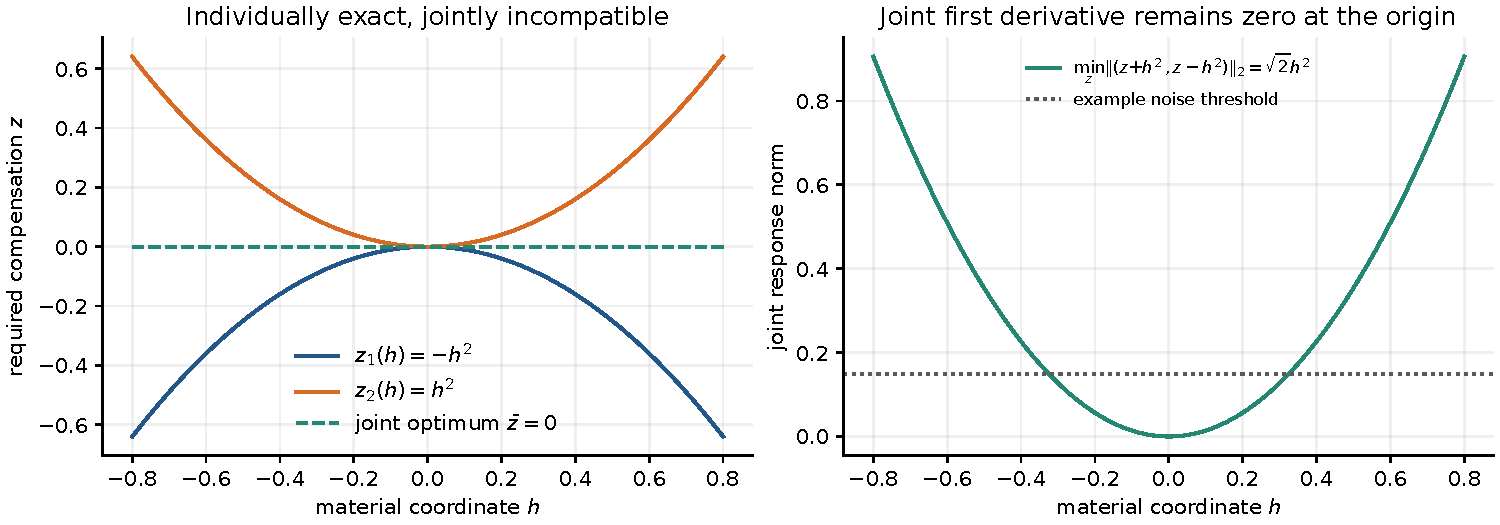
\includegraphics[width=\linewidth]{figures/shared_compensation.pdf}
\caption{共享补偿的解析反例。两个单独观测分别允许精确补偿，但同一材料不能同时采用两个相反的补偿。这不是 Maxwell 实验；它定义了 E2 要寻找或否证的物理机制。}
\end{figure}

\subsection{可计算的联合补偿分歧公式}
在某一阶 $n$，假定所有采集已共享相同的低阶材料系数，第 $a$ 个采集的本阶响应为 $A_a z+b_a$，且各 $A_a$ 满列秩。各采集按正确独立噪声块白化，使用同一物理强坐标 $z$；噪声相关时须先按联合协方差整体白化后重新建立分块。本阶强坐标可在声明内点无约束变化。定义
\[
H_a=A_a^*A_a,\qquad z_a=-A_a^+b_a,\qquad
c_a=(I-P_{A_a})b_a,\qquad
\bar z=\left(\sum_aH_a\right)^{-1}\sum_aH_az_a.
\]
则有精确分解
\begin{equation}
\min_z\sum_a\|A_az+b_a\|^2
=\sum_a\|c_a\|^2+\sum_a\|z_a-\bar z\|_{H_a}^2.
\label{eq:compensation-disagreement}
\end{equation}
证明只需写 $A_az+b_a=A_a(z-z_a)+c_a$，利用两项正交，再作加权平方完成。第一项是各采集本来就不可补偿的部分；第二项是它们要求的强材料补偿互相冲突产生的新约束。即使每个 $c_a=0$，第二项仍可为正。

这一加权最小二乘恒等式本身是成熟代数；多频、多照明共享同一材料也是成熟联合反演建模。可争取的新增贡献是最早冲突阶、有效材料位移区间和采集揭示能力的可计算预测。值得研究的 Maxwell 内容是 $b_a$ 由真实多次散射递推生成，并且所有采集必须共享同一材料补偿。式 \eqref{eq:compensation-disagreement} 可在未计算完整路径和 posterior 的情况下预测哪些新采集会破坏当前弱材料变化，是比“再做一次动态 SVD”更明确的候选物理机制。若不同采集早在更低阶就需要不同补偿，应在最早冲突阶应用，不能把各自独立走出的低阶路径混合。

\subsection{从几何到统计的局部下界}
若两材料 $m_0,m_h$ 的噪声形状白化响应距离 $d_h\le C|h|^p$，任务差异 $\Delta_\varphi\ge c|h|^s$，则 Gaussian 数据模型的 KL 为
\[
D_{\rm KL}(P_{m_h}\|P_{m_0})=\frac{d_h^2}{2\sigma^2}.
\]
取 $h=a\sigma^{1/p}$ 且 $a$ 足够小，可使总变差小于固定常数。由两点检验归约，任意任务估计器的这两个模型最大平方风险至少为
\[
\frac{\Delta_\varphi^2}{8}
\bigl(1-\|P_{m_h}-P_{m_0}\|_{\rm TV}\bigr)
\gtrsim \sigma^{2s/p}.
\]
证明是以估计值距两个任务值的最近者构造检验；分类错时平方误差至少 $\Delta_\varphi^2/4$，再用两模型平均检验错误下界。它是成熟 Le Cam 方法的条件应用，不是全局 Bayes 风险率。其作用是把已验证的 Maxwell 补偿弧转成任务无法任意准确的统计见证。


\section{概率体积：响应阶、任务阶与先验质量阶必须分开}
\label{sec:volume}

\subsection{单条相容路径不够定义概率体积}
一条高维材料空间中的光滑曲线通常具有零 prior 质量。由一条弧上的 $F(m(h))-F(m_0)\sim ch^p$，不能直接推出完整 posterior 的分支质量。必须建立一个有正测度的局部 chart/锥邻域，控制横向方向、角向零点、强变量条件积分、远分支和归一化。

同理，式 \eqref{eq:profile} 是几何补偿中心，不自动等于 noisy likelihood 的真正 profile 最优点，也不等于把强变量积分掉后的条件均值。若使用它作 Laplace 中心，须证明强 Hessian 稳定、局部唯一性及随噪声的余项控制；其 determinant/prior 体积因子不能丢。

\subsection{命题三：一个可严格证明的分层条件模型}
以下命题刻意限制到可验证模型，而不将一条 Maxwell 弧直接升级成 Full66 定理。

\begin{theorem}[任务分辨的接缝质量尺度]
\label{thm:scaling}
假设材料 prior 由 $m_0$ 的正质量原子 $w_0\delta_{m_0}$ 与一条真实一维材料分支组成。分支坐标 $h\in(0,h_0]$ 的 prior 为
$a(h)h^{\alpha-1}dh$，$a(h)\to a_0>0,\alpha>0$。固定噪声形状白化后
\[
\bar F(m(h))=\bar F(m_0)+c h^p+o(h^p),\quad c\ne0,
\]
\[
\varphi(m(h))-\varphi(m_0)=b h^s+o(h^s),\quad s\ge0.
\]
数据为 $\bar y=\bar F(m_0)+\sigma\xi$，$\xi$ 固定在一个有界集合中。假设缩放后的 evidence 被积函数与中心化任务被积函数分别具有统一可积支配；远离接缝的 evidence 贡献为 $o(\sigma^{\alpha/p})$，中心化任务贡献为 $o(\sigma^{(\alpha+s)/p})$；总归一化由原子项主导。则
\begin{align}
Z_{\rm br}(\sigma,\xi)
&=\sigma^{\alpha/p}\{a_0 I_{\alpha,p}(\xi)+o(1)\},\\
P({\rm br}\mid y)&=O(\sigma^{\alpha/p}),\\
T_\varphi(y)-\varphi(m_0)&=O(\sigma^{(\alpha+s)/p}),
\label{eq:three-exponents}
\end{align}
其中
\[
I_{\beta,p}(\xi)=
\int_0^\infty t^{\beta-1}
\exp[-\tfrac12\|ct^p-\xi\|^2]\,dt.
\]
若领先常数非零，$O$ 可加强为对应的渐近等价。典型分支宽度为 $h=O(\sigma^{1/p})$。
\end{theorem}
\begin{proof}
在分支 evidence 积分中令 $h=\sigma^{1/p}t$，测度因子变成
$\sigma^{\alpha/p}a(\sigma^{1/p}t)t^{\alpha-1}dt$，likelihood 逐点趋于定义中的指数函数。由统一支配与远分支控制可交换极限和积分。原子项为
$w_0e^{-\|\xi\|^2/2}$，有正的 $O(1)$ 极限，因此除以总 evidence 得分支质量阶。中心化任务分子额外乘 $b\sigma^{s/p}t^s+o(\sigma^{s/p})$，再除以同一归一化即可。
\end{proof}

对多维分支，可在极坐标下得到类似结果，但需要领先齐次响应在声明角域上统一非退化。例如 $w\in\R^d$，$\|P_p(w)\|\asymp\|w\|^p$，prior 径向指数为 $d+\beta-1$，则 $\alpha=d+\beta$。若强变量先积分，必须证明其 determinant、先验及正则噪声因子一致受控；不同 strata 的强方向维数不同会改变 evidence 的额外幂次。上述命题不能省略这些条件直接覆盖真实 Full66。

该命题使用成熟的奇异 Laplace 缩放思想。\refl{L15} 新颖性候选在于：用真实 Maxwell 补偿得到可验证的 $p$、有效局部域和常数，并区分材料任务的 $s$，而不是仅观察一个三次 decoder。

\subsection{R6 与真正 Maxwell 高阶弱性的区别}
\begin{longtable}{p{.29\linewidth}p{.19\linewidth}p{.2\linewidth}p{.24\linewidth}}
\toprule
局部机制 & $(p,s,\alpha)$ & 分支质量 & 材料任务漏项\\
\midrule
R6 三次 decoder seam，正原子主导 & $(3,3,1)$ & $\sigma^{1/3}$ & $\sigma^{4/3}$\\
材料正则弧，物理补偿至三阶，正原子主导 & $(3,1,1)$ & $\sigma^{1/3}$ & $\sigma^{2/3}$\\
事件跨分支跳变 & $(p,0,\alpha)$ & $\sigma^{\alpha/p}$ & 同阶 $\sigma^{\alpha/p}$\\
无原子、连续分支主导 & 同样的局部 $p,s$ & 可为 $O(1)$ & 通常条件变化尺度 $\sigma^{s/p}$\\
\bottomrule
\end{longtable}
第二行是条件理论，不是 R6 已证实的现象；真实 regular 材料 prior 通常并无 $m_0$ 原子，第四行往往更相关。对某个对称分支，材料均值的领先项还可能因奇偶性相消，均值误差很小而方差或事件仍大，因此同时评价均值、协方差和材料事件。

\begin{figure}[htbp]
\centering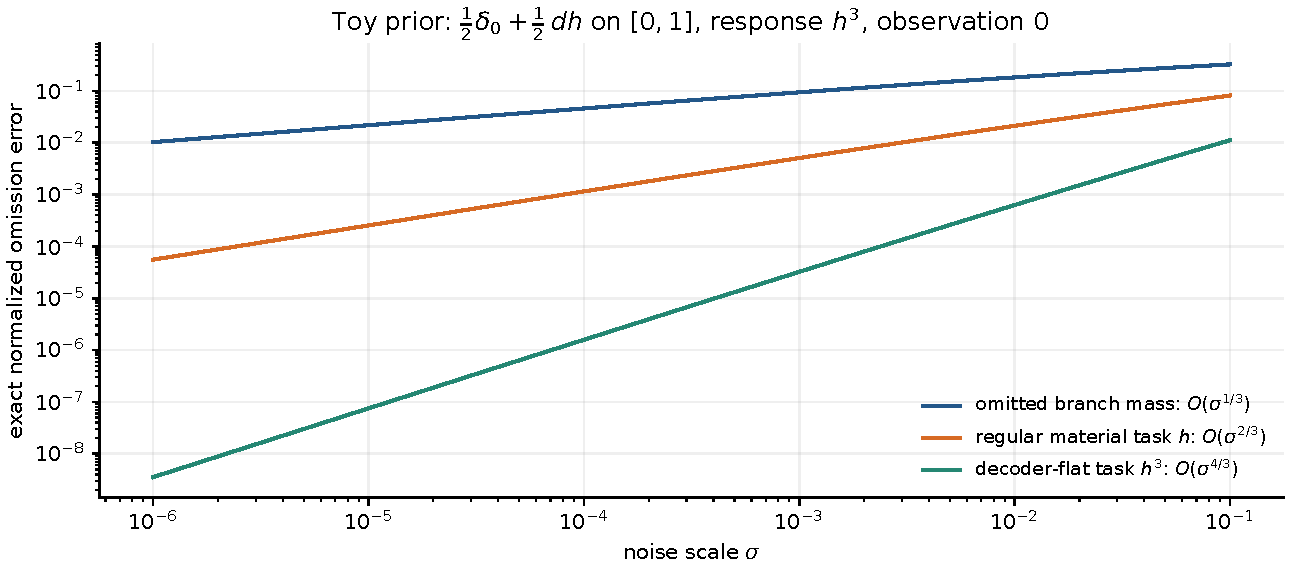
\includegraphics[width=.95\linewidth]{figures/atom_task_scaling.pdf}
\caption{正原子主导的受控一维模型。相同三阶响应下，分支质量、正则材料任务和 decoder 平坦任务有不同误差阶。图中是归一化积分的解析结果，不能外推为 Full66 或普通无原子材料先验的规律。}
\end{figure}

\subsection{三个阻止错误外推的反例}
\textbf{无原子。} $h\sim\mathrm{Uniform}[0,1]$，$F(h)=h^p$，观测零附近。posterior 全部位于连续分支，分支概率恒为 1；只能说其宽度缩小。$\sigma^{1/p}$ 质量说法不成立。

\textbf{角向退化产生对数。} $(u,v)\sim\mathrm{Uniform}[0,1]^2$，$F=uv$。有
\[
P(uv\le\sigma)=\sigma+\sigma\log(1/\sigma),\quad0<\sigma<1.
\]
证明为分别积分 $u\le\sigma$ 和 $u>\sigma$ 时允许的 $v$ 长度。一条固定方向的二阶响应，不能捕获靠近坐标轴的体积与对数因子。

\textbf{固定离开模型的 residual。} 若观测与所有局部响应保持不随 $\sigma$ 缩小的偏离，likelihood 可能由边界、远分支或另一鞍点主导；固定标准化创新假设失效。不能把一个局部 seam 的小噪声公式解释为全局 posterior 率。

\subsection{真正必要的体积是什么}
需要计算的是对任务积分有影响的 $L_y\,d\mu_0$，以及漏掉区域的可控贡献。若只求一个有界材料功能，不必恢复每个 latent 的联合 density；若要多个物理模式的概率、置信区域或主动测量，必须知道不同材料分支的质量；若报告“latent $Q>0.5$”这样的非材料事件，还必须保留 $K_G$。不存在对所有任务都可以删除的“无用概率体积”。

\section{Task-Conditional Observability：一个一阶响应和一个完整任务信息对象}
\label{sec:taskinfo}

\subsection{不要把敏感性、剩余风险和新增信息混成一个量}
对向量任务 $\varphi(M)$，至少有三个对象：
\[
T_\varphi(y)=\E[\varphi\mid y],\qquad
V_\varphi(y)=\Cov(\varphi\mid y),\qquad
D_yT_\varphi(y).
\]
第一个是估计，第二个是条件不确定性，第三个是对当前数据的局部响应。高敏感性不意味着大风险下降；零导数也不意味着完全无信息。对于新采集 $a$，真正的实验信息还涉及尚未见到的 $Y_a$。

\subsection{Gaussian 任务响应及层内/层间分解}
在允许微分与积分交换的可积条件下，经典 Gaussian identity 给出
\begin{equation}
D_yT_\varphi(y)=
\Cov(\varphi(M),F(M)\mid y)\Gamma^{-1}.
\label{eq:task-score}
\end{equation}
由求导归一化 likelihood 可直接证明：score 是
$\Gamma^{-1}(F(M)-\E[F\mid y])$，与 $\varphi$ 相乘再取期望即可。它允许材料原子，不要求 prior 有 Lebesgue density；这已被一般 conditional-mean identity 覆盖。\refl{L17}

定义一阶白化任务响应
\[
B_\varphi(y)=\Cov(\varphi,F\mid y)\Gamma^{-1/2}.
\]
对互斥的材料分支标签 $S$，
\[
\Cov(\varphi,F\mid y)
=
\sum_s w_s\Cov_s(\varphi,F)
+
\Cov_{S\mid y}\big(\E[\varphi\mid S,y],\E[F\mid S,y]\big).
\]
第一项是分支内响应，第二项是分支质量迁移的代数贡献。向量或矩阵的两项通常不正交，范数比例不构成可加的信息百分比。R6 的约 28\% 是 between-source 导数范数比；source 的材料像可重叠，因此更不能直接称为 28\% 的物理模式信息。\refe{R6-A}

在局部线性 Gaussian 近似，$\varphi\approx Lm$，
\[
B_\varphi\approx L C_{\rm post}J^*\Gamma^{-1/2}.
\]
任务相关方向由 $L$、posterior covariance、$J$ 及噪声共同决定，不只是 $J^*J$ 的最大特征向量。此基本原则已有 goal-oriented inverse 的最优低秩理论。\refl{L7}

\subsection{命题四：完整的新增测量任务信息}
令当前 posterior 为 $\mu_y$，新采集的条件分布为 $p_a(dz\mid m)$。定义中心化条件期望算子
\[
\mathcal C_{a,y}:L^2_0(\mu_y)\longrightarrow L^2_0(p_a(\cdot\mid y)),
\quad
g\longmapsto \E[g(M)\mid y,Y_a].
\]
其任务信息算子为
\[
\mathcal O_{a,y}=\mathcal C_{a,y}^*\mathcal C_{a,y}.
\]
这是真正作用于材料函数的算子，不必把材料函数线性化成一个方向。

\begin{theorem}[任务信息与 Bayes 风险；成熟条件期望原理]
\label{thm:task-information}
$\mathcal O_{a,y}$ 自伴、半正定，且 $0\preceq\mathcal O_{a,y}\preceq I$。对标量平方任务，
\begin{align}
\langle\varphi-\E_y\varphi,\mathcal O_{a,y}(\varphi-\E_y\varphi)\rangle
&=\Var_{Y_a\mid y}\big(\E[\varphi\mid y,Y_a]\big)\\
&=\Var(\varphi\mid y)-\E_{Y_a\mid y}\Var(\varphi\mid y,Y_a).
\label{eq:task-bayes-reduction}
\end{align}
向量任务的对应矩阵
$\mathcal I_{a,\varphi}(y)=\Cov_{Y_a\mid y}(\E[\varphi\mid y,Y_a])$
为平均后验任务 covariance 的精确下降。
\end{theorem}
\begin{proof}
条件 Jensen 给 $\|\mathcal C g\|_2\le\|g\|_2$，故 $\mathcal C^*\mathcal C$ 是正收缩。第一等式来自算子定义；第二等式为条件全方差公式。向量情形逐个二次型应用标量结果。
\end{proof}

该算子可以称为本问题的 task-information 对象，但不能宣称它独立于成熟 Bayesian decision theory。它的 Maxwell 特征全部进入 $p_a(dz\mid m)$ 和 $\mu_y$。可能的新贡献是利用真实物理补偿结构计算它，而不是给它取名。

如果新增观测重复旧响应且噪声趋零，它无法区分旧 exact fibers 内的材料。新采集沿旧 fiber 变化，才可能降低给定旧无噪响应后的材料任务方差；对指定平方任务，平均风险严格下降当且仅当相应条件任务均值随新增观测非恒定。单次观测的 posterior 方差不保证下降。材料可区分性与任务条件依赖共同连接多解探索和测量设计。\refl{L18,L19}

\subsection{一阶协方差不是完整的信息：精确反例}
设当前材料只有三个值，
\[
M\in\{-1,0,1\},\qquad P=(1/4,1/2,1/4),\qquad
\varphi(M)=M^2,
\]
新观测为 $Y_t=\sqrt tM+N$，$N\sim N(0,1)$。因为对称性，
$\Cov(M^2,M)=0$。但
\[
\E[M^2\mid Y_t=z]
=
\frac{e^{-t/2}\cosh(\sqrt t z)}
{1+e^{-t/2}\cosh(\sqrt t z)}
\]
对每个 $t>0$ 都不是常数，所以真正任务信息严格为正。展开得
\[
\E[M^2\mid Y_t=z]=
\tfrac12+\tfrac{t}{8}(z^2-1)+O(t^2),
\qquad
\mathcal I_{t,\varphi}=\frac{t^2}{32}+o(t^2).
\]
以上点态展开配合 Gaussian 可积余项控制给出方差渐近。这说明零一阶协方差不能断言任务无信息。对新采集
$Y_{a,t}=\sqrt t F_a(M)+\eta_a$，$\eta_a\sim N(0,\Gamma_a)$，
新增噪声条件于材料与旧数据独立。定义
\[
B_{a,\varphi}(y)=\Cov_{\mu_y}(\varphi,F_a)\Gamma_a^{-1/2}.
\]
在相应矩与微分条件下，
$\mathcal I_{a,t,\varphi}=tB_{a,\varphi}B_{a,\varphi}^*+o(t)$。
这里使用新采集而非旧 $F$ 的协方差。上述对称例的一阶项为零，必须保留更高阶或有限信号模型；若新增噪声与旧数据相关，应使用完整条件通道 $p_a(dz\mid m,y)$。

\begin{figure}[htbp]
\centering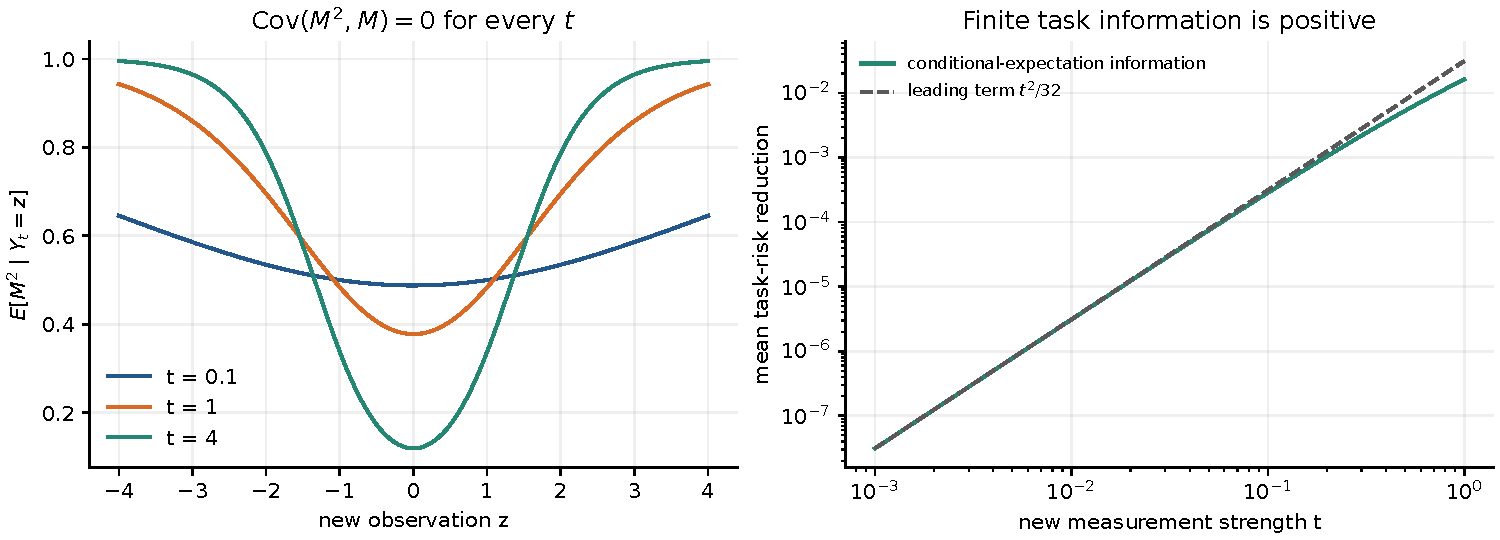
\includegraphics[width=\linewidth]{figures/zero_covariance_information.pdf}
\caption{三点材料先验的解析反例：一阶任务协方差为零，但新观测对平方任务的信息严格为正。右图为一维 Gaussian 求积与小信号公式；未运行 Maxwell。}
\end{figure}

\subsection{为什么不合格 posterior provider 仍能改善材料成像}
平方损失的标准分解为
\[
\E\|\widehat a(Y)-M\|^2
=
\E\|T_M(Y)-M\|^2+
\E\|\widehat a(Y)-T_M(Y)\|^2.
\]
一个 provider 即使不能给出正确联合密度，也可能输出与 $T_M$ 有关的有用特征；下游监督 head 可使用这些特征降低第二项。R4 的普通 Gaussian 与 Flow 融合几乎同样好，符合这种解释，但没有测到真正的 $T_M$，不能从现有数据精确分解其 Bayes excess。

进一步，posterior mean 通常不在 decoder image 内。要求 Maxwell-consistent representative 时，可以在可行材料中求
\[
m_{\rm rep}\in\argmin_{m\in\mathcal A(y)}
\E_{\mu_y}\|m-M\|_{W_M}^2,
\]
等价于在所声明的可行集合 $\mathcal A(y)$ 中投影 posterior mean；这与均值、MAP、样本是不同输出。$\E F(M)\ne F(\E M)$ 也意味着均值图散射不相容未必说明条件均值错误。

\subsection{物理特征的计算价值不等于新增观测信息}
固定已知 forward、prior 和训练资产，若 current、Jacobian、KKT 或其它特征为 $A(Y)$，则
\[
\sigma(Y,A(Y))=\sigma(Y),\qquad
\E[\varphi(M)\mid Y,A(Y)]=\E[\varphi(M)\mid Y].
\]
第一式直接来自 $A(Y)$ 的可测性，第二式来自条件期望的唯一性。引入条件于 $Y$ 独立于材料的算法随机种子，也不会增加真实材料信息。这是数据处理原则的直接应用，不是新的 Maxwell 定理。

因此 E5 所谓“超出 raw measurement 的增量”只能指：有限数据、有限容量、有限训练或有限物理预算下，材料统计更容易被估计，或者达到同一精度更便宜；不能声称确定性物理特征增加了原始数据的 Shannon 信息。若另有新采集、未知模型校准或外部 prior 信息，须显式加入观测/条件模型。

这一区别同样适用于任务导向物理计算：继续计算 current 或 Jacobian 可以降低已有材料信息的数值提取误差，真实新增采集则可能减少材料的统计不确定性。两种费用可以联合优化，但不是同一种信息增益。

\subsection{没有合格 Full posterior sampler 时如何估计}
可以采用三条有不同资格的路径。

第一，在低维非均匀条件模型中用可信全域积分计算 $T,V,B,\mathcal I$，检验理论与误差，不把条件切片冒充 Full66 边缘。第二，利用 prior predictive 模拟对 $(Y,\varphi(M))$ 做 proper supervised regression，直接估计任务条件矩；这是风险学习，需独立任务 MSE 与事件校准，不能据此认证全部 posterior。第三，多中心局部 Gaussian/stratified mixture 可作计算近似，但权重、外部质量及高阶盲点均须单列。

R6 B6 的高 SNR 条件矩回归失败提示：原始矩相减再乘 $\sigma^{-2}$ 会放大回归误差。使用同 fold 的中心化目标、标准化观测、直接任务回归或双样本校正可以改善数值条件，但导数一致性仅是必要诊断之一；一个错误模型也可能内部自洽。\refe{R6-B}

材料均值、局部相事件、空腔事件、covariance、后验预测散射和工程功能量必须分别评价。均值很准不保证结构存在概率准；某个任务 covariance 小也不保证另一个非线性任务容易判断。


\section{任务精度怎样决定 Maxwell 与 Jacobian 的精度}
\label{sec:accuracy}

\subsection{不需要稳定每个弱特征向量}
在已声明的局部线性 Gaussian 模型中，把观测白化，令
\[
K=\Lambda+J^*J,\quad C=K^{-1},\qquad
\widehat J=J+E,\quad \widehat C=(\Lambda+\widehat J^*\widehat J)^{-1},
\]
其中 $\Lambda\succeq aI$，$a>0$，是固定真实 prior precision 或明确声明的局部正则近似。对线性任务 $Lm$，
\[
\Delta K=J^*E+E^*J+E^*E,\qquad
\widehat C-C=-\widehat C\,\Delta K\,C.
\]
故
\begin{equation}
\|L(\widehat C-C)L^*\|
\le
\|L\widehat C\|\,\|\Delta K\|\,\|CL^*\|,
\quad
\|\Delta K\|\le 2\|J\|\|E\|+\|E\|^2.
\label{eq:task-cov-error}
\end{equation}
该界没有 weak spectral gap 的分母。特征向量在近重根处可以大幅旋转，但 $LC L^*$ 仍稳定。如果只需少数任务，可求 task dual $CL^*$，再针对其实际受影响方向验证 $E$；不必把整个 $J$ 的每个弱 eigenvector 算准。

同一线性问题的均值满足
\[
\widehat m-m=
\widehat C\{E^*(y-Jm)-\widehat J^*Em\}
\]
（以相同中心和 prior 线性项定义）。因此任务误差取决于误差在 residual 和 task dual 上的作用，不只取决于 $\|E\|$。这是标准 resolvent/正规方程扰动的任务化应用；只有实际得到廉价方向误差估计，才形成算法收益。

它不能直接认证 nonlinear、多模态、分层 Full posterior。若 $\Lambda$ 只是数值 damping，则相应 covariance 不是自动的 Bayesian covariance；若 posterior 远分支改变 task，局部 Hessian 再精确也无济于事。

\subsection{命题五：可用于在线停止的中心化任务误差界}
\begin{theorem}[中心化积分证书]
\label{thm:task-certificate}
设已计算覆盖域 $C$，$B_b$ 是 $C^c$ 的可数可测分割，并要求下述求和有限。令输出为任意 $t$。若已有严格数值界
\[
Z_y\ge Z_L>0,\qquad
\left|\int_C(\varphi-t)L_y\,d\mu_0-\widehat Q_C\right|\le e_C,
\]
并且每个遗漏块上
\[
|\varphi(m)-t|\le a_b,\qquad
\int_{B_b}L_y\,d\mu_0\le U_b,
\]
则
\begin{equation}
|T_\varphi(y)-t|
\le
\frac{|\widehat Q_C|+e_C+\sum_ba_bU_b}{Z_L}.
\label{eq:centered-certificate}
\end{equation}
这里 $e_C$ 必须包括覆盖域内的求积、forward 数值误差及所用 prior 近似误差。
\end{theorem}
\begin{proof}
把 $Z_y(T_\varphi-t)=\int(\varphi-t)L_y\,d\mu_0$ 按 $C$ 及遗漏块分解，对每块取绝对值界，再用 $Z_y\ge Z_L$。
\end{proof}

如果 $t=\widehat N_C/\widehat Z_C$ 且同一求积规则计算中心化分子，通常 $\widehat Q_C=0$；仍须对真实积分的 defect 给 $e_C$。一个材料均值任务可能有很小的 $a_b$，而事件任务 $a_b$ 接近 1，这才是任务积分可能节省的严格入口。该不等式不是凭有限节点自动获得的证书。

例如在块 $B_b$ 上若有先验质量 $p_b$、可验证的 residual 下界 $\underline r_b$，则
\[
U_b\le p_b e^{-\underline r_b^2/2}.
\]
无 residual 下界时，$U_b\le p_b$ 虽然正确，却在高 SNR、evidence 很小时可能完全无用。先验 tail 小不自动意味着 posterior tail 小。

\subsection{同 prior 下的任务加权 likelihood 误差}
对 $\mu\propto e^{-\Phi}\mu_0$、$\widehat\mu\propto e^{-\widehat\Phi}\mu_0$，置
$\delta=\Phi-\widehat\Phi$、$\widehat T=\E_{\widehat\mu}\varphi$。精确有
\begin{equation}
T-\widehat T=
\frac{\E_{\widehat\mu}[(\varphi-\widehat T)(e^{-\delta}-1)]}
{\E_{\widehat\mu}e^{-\delta}}.
\label{eq:weighted-potential}
\end{equation}
若可验证 $|\delta(m)|\le b(m)$，
\[
|T-\widehat T|
\le
\frac{\E_{\widehat\mu}[|\varphi-\widehat T|(e^{b}-1)]}
{\E_{\widehat\mu}e^{-b}}.
\]
该式体现任务振幅与物理误差的乘积。若右侧期望仍需未知 posterior 或难以求积，它只是理想误差表达；不能称作已实现的便宜停机器。PDE potential 误差传递到 posterior 与函数量已有成熟理论。\refl{L21,L22}

\subsection{Maxwell 残差与 adjoint 能提供什么}
对状态方程 $Lu=b$，近似状态 $\widetilde u$ 的 residual 为 $r_u=b-L\widetilde u$；观测为 $Su$。若
$L^*z=S^*a$，则
\[
a^*(Su-S\widetilde u)=z^*r_u.
\]
若仅有近似 dual $\widetilde z$，其 residual
$r_z=S^*a-L^*\widetilde z$，并有已认证稳定常数
$\|L^{-1}\|\le\beta^{-1}$，则
\[
\left|a^*S(u-\widetilde u)-\widetilde z^*r_u\right|
\le \beta^{-1}\|r_z\|\,\|r_u\|.
\]
这给 task-weighted 输出误差接口。若全白化输出误差界为 $\delta_f$，则
\[
|\Phi-\widehat\Phi|
\le\|\widehat f-y_w\|\delta_f+\tfrac12\delta_f^2
\]
在 $\Phi=\frac12\|f-y_w\|^2$ 约定下成立。

关键成本问题是 $\beta$、dual 及全域覆盖是否便宜。计算精确最小奇异值可能与原求解同样贵；passivity 不会自动给紧的 resolvent 界；近共振时界可能爆炸。可用离线 reduced-basis 稳定下界、局部参数盒包络或已付费 LU 的误差估计，但应把建立它们的费用列入账本。若最终还需为每节点重新 Full Maxwell，便没有证明“证书更便宜”。

\subsection{不能由局部样本推出普遍全域证书}
对没有任何已知全局正则常数的光滑 black-box forward 类，任何仅查询有限点和有限阶导数的算法都可能被反例击穿：在所有已查询点之外选择一个有正 prior 质量的小区域，用光滑 bump 改变 forward，使其产生与 $y$ 相容且任务值不同的新模式；所有已有查询保持不变，而 posterior task 可以改变。自适应查询也可按相同 transcript 构造。

这不是任意固定 Maxwell 材料类的不可能性定理，因为 Maxwell 方程限制了可实现 forward。它说明普遍证书必须利用明确的物理参数类、全域稳定性/覆盖或尾部假设。R6 的局部 GH 加密尚未提供这些信息。\refe{R6-A}

\subsection{四种停止规则的资格}
\begin{longtable}{p{.24\linewidth}p{.42\linewidth}p{.26\linewidth}}
\toprule
规则 & 可以说明什么 & 不能说明什么\\
\midrule
GT/oracle 风险停止 & 离线潜力上界 & 在线可执行性。\\
学习的风险预测器 & 同分布独立集的群体预测误差 & 给定 $y$ 的点态 posterior 积分界。\\
校准或 conformal 规则 & 满足交换性等条件下的边际覆盖 & 任意分布移位、任意自适应停止的条件覆盖。\\
式 \eqref{eq:centered-certificate} 的严格界 & 在已声明模型/覆盖/误差条件下的任务误差 & 未覆盖模型、未知外部分支的正确性。\\
\bottomrule
\end{longtable}
已有 task-driven conformal inverse work 已研究任务不确定性和测量停止，不能把边际校准重新命名成全局 Bayesian 证书。\refl{L20}

\subsection{预算分配与 break-even}
在已有分块 prior 质量 $p_b$ 的 stratified Monte Carlo 中，令
$\psi=(\varphi-T)L_y$，块内标准差为 $s_b$，每样本费用为 $c_b$。在一阶 ratio 近似成立时，
\[
\Var(\widehat T)\approx
Z_y^{-2}\sum_b\frac{p_b^2s_b^2}{n_b}.
\]
给定总费用，Lagrange 乘子给
\[
n_b\propto \frac{p_bs_b}{\sqrt{c_b}},
\qquad
C_{\min}\approx
\frac{\left(\sum_bp_bs_b\sqrt{c_b}\right)^2}{Z_y^2\eps_{\rm MC}^2}.
\]
这是成本加权 Neyman 分配的应用，$T,s_b,Z_y$ 若未知，pilot plug-in 只有近似资格；完整 finite-sample 保证要额外控制 pilot 与停止的适应性。

实际总误差应分为
\[
e_{\rm task}\le
e_{\rm covered\;integration}
+e_{\rm omitted\;branches}
+e_{\rm forward}
+e_{\rm prior/model},
\]
各项预算预先分配，例如参考误差至多容忍度的 $1/5$。Jacobian 误差若只影响 proposal 而最终以真 likelihood 正确修正，主要影响效率；若进入 approximate target 或停止证书，就必须进入偏差预算。

有离线训练/建库费用时，至少达到
\[
N_{\rm break-even}>
\frac{C_{\rm off,new}-C_{\rm off,base}}
{c_{\rm online,base}-c_{\rm online,new}}
\]
且分母为正，才可能获得摊销收益；前提仍是两者达到同样任务误差。教师、reference、缓存建立、失败求解和计时 I/O 都不能免费化。

\section{三个机制不同、可以实现的算法方案}
\label{sec:algorithms}

\subsection{方案一：材料补偿 chart 与多解探索}
\textbf{原始问题：} 在正确 prior 的材料空间内，寻找具有实际材料距离而仍数据相容的候选，并预测不同采集如何破坏补偿。历史动态 SVD 只给一阶方向；四段轨迹没有定义概率密度；直接 current 路径可能不对应共享材料。

\textbf{构造：} 在材料 regular strata 建立有限域 response-aligned charts，使用命题 \ref{thm:jets} 计算各方向的强补偿与剩余系数；在 rank/seam 变化处开新 chart。选择方向的依据是可行任务位移、响应界及预计物理费用，不是固定 bottom-$k$ 名称。

\begin{tcolorbox}[title={算法 1：compensated material chart}]
输入：合法材料中心、prior/decoder、采集、材料度量、任务、预算。\\
1. 分析 $DG$，验证有限同材料 gauge；只在确认后消去，记录材料 prior 权重。\\
2. 在材料正交 frame 上求一阶强/弱结构，选定可行 $v,U$，归一化材料弧。\\
3. 用同一背景 LU 递推到三阶；给每个系数及余项的误差状态。\\
4. 求低阶/高阶/余项共同允许的非空区间；区间为空时使用普通 nonlinear corrector。\\
5. 以预测器提议端点，用真实 Maxwell 校正/验证；保留失败和实际费用。\\
6. 达到 seam、边界或采集改变时更新 chart；分离等材料副本与真正材料候选。\\
7. 若要 posterior，另计算合法 proposal 密度与 prior/chart 权重，做 MH/IS 或可信求积；否则仅交付候选及相容性。
\end{tcolorbox}

\textbf{适用条件与复杂度：} 局部强响应满秩、可行材料 chart、状态可逆；每方向 $p$ 阶约需 $pP$ RHS 及低阶 Green actions，另有初始强基构造、有限端点新 LU。$N$ 个内部自由度的 dense LU 为 $O(N^3)$、每 RHS 为 $O(N^2)$；矩阵自由/稀疏 3D 改用实际迭代和预条件费用，不外推固定比例。需缓存场而非保留无限历史 LU。

\textbf{概率接口：} overlapping source images 先把 prior 贡献相加；仅用于覆盖同一材料区域的多个数值 charts 再用 partition of unity 分摊，避免双计。两种“重叠”不能混为一谈。若无法计算 proposal density，不能给出后验权重。

\textbf{强竞争：} 普通 material retraction、Full-J predictor--corrector、nonlinear profile、多起点/RTO、LIS、iTSVD；不能只比较 frozen SVD。决定性实验是 E2 的有限域响应预测及新采集破补偿，再看同费用有效候选或任务距离。

\textbf{失败条件：} 现象全来自 $DG$、真实有限验证不支持高阶工作区间、复杂方法被普通 corrector 覆盖、可行边界截断全部路径。此时暂停其算法优势，不否定有限噪声材料集合存在。原创性来自可验证的 Maxwell 补偿机制与用途；递推公式本身不足。

\subsection{方案二：保留分层材料测度的任务积分}
\textbf{原始问题：} 准确材料均值、事件和预测散射是否需要相同的分支概率精度？历史局部 Gaussian/独立边缘会丢条件核；全局网格则漏窄 likelihood；普通样本数无法直接保证功能误差。

\textbf{构造：} 用 $\mu_0$ 定义正确对象，把原子、regular charts、seam 与遗漏域分别积分；使用中心化任务 defect 及每块 $a_bU_b$ 分配物理预算。可使用方案一的 charts，但没有它也能独立成立，因此这是不同的数值机制。

\begin{tcolorbox}[title={算法 2：task-certified stratified integration}]
输入：有界条件材料模型、任务及容忍度、先验分块、全域覆盖规则。\\
1. 解析保留原子与 exact gauge 质量；为连续块建立 source-CDF 或材料 chart 求积。\\
2. 以独立 pilot 定位窄 likelihood，明确所有未覆盖块及 prior 质量。\\
3. 同时维护 $N,Z,Q=N-tZ$ 的上下界；物理节点携带 forward 误差及费用。\\
4. 计算式 \eqref{eq:centered-certificate}；选 task-weighted 上界最多且可降低的块细化。\\
5. 需要时增加真实 Maxwell、缩小状态误差或搜索外部分支；每步更新总误差预算。\\
6. 仅当总界小于 $\eps_\varphi$ 时认证停止；无可靠包络则输出经验收敛状态，不能自称证书。\\
7. 更换为事件任务后重算振幅与误差，不能继承均值的资格。
\end{tcolorbox}

\textbf{适用条件与费用：} 首先限于 3--4 维、有限支撑或可控 tail 的真实非均匀条件模型。每新材料节点通常需要一次 LU 和全部源 forward；若求导只为自适应坐标，应检查其节省是否覆盖额外 RHS。不存在一般“降到 quotient 就克服维数灾难”的定理。

\textbf{强竞争与原创性：} source-CDF 自适应积分、defensive IS/SMC、RTO、goal-oriented quadrature、CoCoS 的 regular-volume 思路。新贡献必须是 Maxwell 分支结构让可计算任务界更紧，且同精度总费用更低。若只有人工 quintic 原子有优势，适合作为反例/方法附录，不能撑起一般 Maxwell TAP 主文。

\subsection{方案三：任务 dual 控制的物理精度与求解安排}
\textbf{原始问题：} 是否值得再解一次 current、adjoint 或 Jacobian？R6 的 residual 稳定/材料更新稳定规则不是风险证书；KKT 特征替代并未免除已支付的真实 $J$。

\textbf{构造：} 对指定、固定的估计目标，计算 task dual 和 stationarity/状态残差，使计算决策针对输出误差。对于局部强凸目标 $\Psi$，
\[
m_\star-\widehat m\approx-H^{-1}\nabla\Psi(\widehat m),\quad
\varphi(m_\star)-\varphi(\widehat m)
\approx-v_\varphi^*\nabla\Psi(\widehat m),
\quad H^*v_\varphi=D\varphi^*.
\]
可靠余项要求局部 Hessian 下界、Lipschitz 常数及同 basin；该式只控制指定优化器输出的功能误差，不能认证与 Bayes action 的距离。

\begin{tcolorbox}[title={算法 3：task-dual physical work control}]
1. 固定 Direct Probit 或明确目标；声明最终任务是 optimizer functional、学习 head 还是 posterior integral。\\
2. 从已有状态取得 stationarity/state residual，不读取 GT 或未来 full endpoint。\\
3. 只对需要的任务构造 dual，估计 forward、Jacobian、优化未收敛和积分误差。\\
4. 比较继续 current solve、更新 $J$、扩大分支、继续积分的预计误差下降/实际费用。\\
5. 对可认证项用上下界决策；对学习风险项标注预测资格。\\
6. 与相同任务的 Direct Probit、Full-q、低预算强基线同窗口比较，报告离线摊销。
\end{tcolorbox}

A17 的两侧变化可用于分析 current 模型改变对任务均值和 covariance 的影响；不能只看 $\Delta J$ 范数或信息行列式。既有 goal-oriented PDE、Krylov、trust-region 和 DINO 已覆盖广义原则，故该方案当前作为模块，除非产生新的、便宜而严格的 Maxwell task error 机制。\refl{L13,L14,L21}

\subsection{R6 两阶段目标到底哪里不一致}
Uniform 属性 $u$ 与 Gaussianized 属性 $x=\Phi^{-1}(u)$ 描述同一 prior 分布；正确换元后 posterior measure 相同，但 density 的最大点不保持不变。Native 与 Probit 各自坐标 MAP 的不同，不等于其中一个 prior 自动写错。它说明先优化一种坐标密度，再优化另一种坐标密度，没有普遍的最优工作分配理由。

Native warm start 可以帮助找到 basin，也可能把属性推向 box 边界，增加后续 Probit 工作。R6 支持后一机制在当前配置中的描述性解释；Direct Probit 的竞争力使“缩短 Native”更像修复原流程。若未来数据表明 Native 在强非线性或大尺度有稳定 basin 收益，再保留，而不是为两阶段结构辩护。

\subsection{更大二维与三维外推的界限}
三维向量 Maxwell 增加状态分量、网格规模、频率和源数，稀疏/快速迭代的瓶颈与 TM24 dense LU 不同。current RHS 复用可能更有价值，也可能被预条件重建、通信或非正规性主导。必须记录 factorization/preconditioner、RHS、Green matvec、内存、训练、尾部搜索和 end-to-end 时间；只用 $N^3$ 或固定源接收比预测百分比加速不可信。首次理论资格可在 2D 建立；强 TAP 的最终物理论证宜补独立向量 Maxwell 小规模 witness 或清楚限制为 TM 材料研究。


\section{Research Narratives：三条论文如何讲完整}
\label{sec:narratives}

\subsection{Paper A：Nonlinear Maxwell Material Ambiguity under Shared Compensation}
\textbf{A. 起源问题。} 拟由 E2 验证的物理图景是：两幅非均匀、物理合法且确实不同的材料图，在原采集下散射几乎相同；改变照明后其中一组补偿无法维持。单点 Jacobian 只能描述无限小响应，不能告诉人们可隐藏多少实际材料变化，更不能区分 decoder 重复表示。

\textbf{B. 现有方法不足。} current SVD 组织辐射可见性，LIS 组织相对 prior 的 likelihood 变化，RTO 组织正确的随机优化 proposal；它们不自动给出一段可行材料补偿区间的物理解释。高阶散射导数已有，但未经强方向补偿的曲率可能主要是可消去的坐标或材料调整。

\textbf{C. 最小核心思想。} \emph{材料歧义由允许的共同材料补偿及其剩余响应决定；新增采集通过使这些补偿互相冲突而揭示材料。}

\textbf{D. 数学主角。} $(\mu_0,\bar F)$ 上的可行材料 chart、不可补偿 jets $c_n$、有限主导区间，以及联合补偿分歧式 \eqref{eq:compensation-disagreement}。Posterior 体积是第二阶段应用，不与几何见证混同。

\textbf{E. 核心定理。} 当前已可完整证明的，是 current 系数递推、response-aligned 隐函数、联合补偿分歧及条件两点任务下界；这些代数与统计工具有成熟先例。真正有竞争力的中心结果应进一步给出：在被动非均匀 Maxwell 材料类内，由可计算 current/dual 误差控制一段非空可行补偿区间，并预测新增采集下的响应下界。该“有效域与用途”部分目前仍待证明/验证，不能写成已完成原创定理。

\textbf{F. 核心算法。} 方案一：材料正则化、分离 gauge/曲率、低阶 current 递推、强补偿、有限端点验证；以补偿冲突选择新增采集或最有价值的探索方向。概率扩展必须加正确 chart prior 与分支 normalizer。

\textbf{G. 决定性实验。} E1 确认 generic 非均匀材料没有被误判 gauge；E2 在 affine 材料 chart 与原 decoder chart 双重对照中展示：物理高阶项在相同材料位移上超过 decoder-only 预测，且补偿分歧预测新采集的揭示能力。主要比较普通 nonlinear profile/Full-J corrector，不只比较 frozen SVD。

\textbf{H. 最强审稿意见。} “这就是 Lyapunov--Schmidt 和 Born 系列。”“你的三阶来自 quintic。”“为什么不能直接多起点优化？”“只找到几条 arc，它们 prior 质量为零。”“响应不变只是同材料 gauge。”这些质疑都合理；不能用更多网络或更多漂亮图回避。

\textbf{I. 拒稿风险与补救。} 最低必要条件：真实材料距离、无平台控制、同费用强基线、非空有效域、至少一新采集、可复现系数/余项。若加 Bayesian Volume 入标题，必须再有正测度 chart、正确 prior 及可信 branch reference。3D vector witness、实验数据和大域泛化是增强项；但文章若宣称通用向量 Maxwell，向量验证便成为必要项。

\textbf{J. 论文结构。} Introduction 从“单次隐藏、联合揭示”图开始；Theory 先说明三空间和材料度量，再给 current jets、补偿冲突和有效域；Algorithm 给有界 predictor--corrector；Experiments 依次排除 gauge、排除 decoder 曲率、检验采集预测和同费用用途；Limitations 明确局部性及未认证全 posterior。标题不宜在 E3 未通过前加入“Bayesian posterior sampling”。

\subsection{Paper B：Task-Conditional Material Uncertainty in Nonlinear Maxwell Imaging}
\textbf{A. 起源问题。} 同一观测下，材料均值可以稳定而结构存在概率仍不稳定；局部 Jacobian 甚至为零时，来自相邻材料区域的 posterior 权重仍会改变任务。R2--R5-B 又显示不合格 posterior 特征能帮助材料点估计。

\textbf{B. 现有方法不足。} 全 posterior 的统一 KL/TV 目标可能为不重要的 latent 自由度支付费用；单点 sensitivity 又看不到远分支迁移。但任务降维和 Bayes-risk 原则已经成熟，单说“任务比参数重要”不够。\refl{L7,L17--L20}

\textbf{C. 最小核心思想。} \emph{只需精确计算能改变指定材料判断的概率质量，但必须证明遗漏部分对该判断的影响。}

\textbf{D. 数学主角。} 带分支条件核的材料 posterior、$T_\varphi,V_\varphi$、完整任务信息 $\mathcal O_{a,y}$，以及中心化积分误差。$B_\varphi$ 只是一阶近似，不作全信息替身。

\textbf{E. 核心定理。} 条件方差分解和 Gaussian identity 都是先例；条件尺度定理 \ref{thm:scaling} 说明响应阶、prior 阶和任务阶如何组合。可争取的新结果是把真实 Maxwell 补偿的可验证局部结构接到任务误差界，并给出小于整体概率误差要求的实际费用。若仅在人工平台成立，理论范围需限定。

\textbf{F. 核心算法。} 方案二用材料分块、source-CDF/正确 quotient 求积与任务权重控制精度；必要时将可信低维任务量蒸馏到监督估计器。后者输出材料函数，不能称为全 posterior。

\textbf{G. 决定性实验。} E3 同时评价材料均值、第二矩、事件与后验预测散射；对每个任务比较同误差费用与全分支质量费用。E5 再验证真实 Maxwell task structure 是否超出 raw measurement、同容量 global encoder、decoder-only 与同谱随机特征。所有消融须匹配训练，冻结 head 删通道造成的 OOD 降级不算因果证明。

\textbf{H. 最强审稿意见。} “Spantini 已经做过目标降维。”“这就是监督 conditional mean。”“你没有合格 sampler，为什么给概率解释？”“均值好而事件错，究竟解决了什么？”答复必须落在指定任务和可验证误差，不使用“完整不确定性”泛称。

\textbf{I. 拒稿风险与补救。} 最低必要条件：可信低维 reference；至少连续量、二阶矩和事件；物理增量的公平控制；任务误差与分支质量明确分开；成本包含全部物理。若决定只写高维风险成像，删除 posterior/calibrated UQ 主张，集中独立风险与 Maxwell 特征作用，不能让未校准 density 承担理论解释。

\textbf{J. 论文结构。} Introduction 展示“同数据，不同任务精度需求”；Theory 给双重条件分解、任务响应与高阶盲点，再给误差预算；Algorithm 展示一套自然使用该误差的积分/估计过程；Experiments 展示同一 posterior 下不同任务的成本曲线和强基线；Limitations 区分条件模型与 Full66。标题中保留 Task-Conditional，不宜宣称已建立全局 observability 新学科。

\subsection{Paper C：Goal-Oriented Maxwell Computation for Material Inference}
\textbf{A. 起源问题。} 物理优化器花费大量工作继续下降其目标，最终材料任务风险却不改善；R6 减少 Native 能节时，而普通 Direct Probit 同样有竞争力。

\textbf{B. 现有方法不足。} 普通优化 residual 不直接控制学习 head 或 posterior task；但 goal-oriented FEM、trust-region、Krylov、delayed acceptance、DINO/LazyDINO 已有相当完整的计算理论。缺口不在“用任务控制计算”这个原则。\refl{L12--L14,L21--L23}

\textbf{C. 最小核心思想。} \emph{只为仍能改变最终材料任务且误差尚未受控的物理动作支付计算。}

\textbf{D. 数学主角。} 可计算的 task dual、状态与 Jacobian defect、局部/全域误差预算。KKT feature 只是一种表示近似，不能代替上述对象。

\textbf{E. 核心定理。} 式 \eqref{eq:task-cov-error} 与 dual residual 是标准数值分析。需要一个 tight、低于重复 Full Maxwell 成本的 Maxwell-specific 估计器，并在真正在线决策中保持任务误差；目前没有这样的实验资格。

\textbf{F. 核心算法。} 方案三，但只能在声明输出类型及误差资格后启动。对 learned head 需要其局部输出敏感性；对 posterior 积分需分支/evidence 控制；对 optimizer functional 只能保证同一目标的未收敛误差。

\textbf{G. 决定性实验。} E4 同窗口、同对象、同目标、同特征比较 Direct Probit、原两阶段、Low-q/Full-q 及新停止器；重复窗口并报 RHS/LU，防止线程/负载改变产生伪速度。若 posterior sampler 是任务对象，再比较正确 RTO/DA；点估计方法与 sampler 不使用不匹配的输出指标硬排名。

\textbf{H. 最强审稿意见。} “你只是删除了冗余优化。”“闭合特征没有省真正的 J。”“Direct Probit 更简单。”“你的停止需要 GT。”“离线 surrogate 费用没有回本。”这些都是当前必须接受的质疑。

\textbf{I. 拒稿风险与补救。} 当前独立主线 NO-GO。只有在线误差与总成本共同过强基线，且机制超出常规优化修复，才重新考虑独立论文；不通过时保留为 B 的工程组件。

\textbf{J. 论文结构。} 如果将来成立，以具体错误预算冲突开篇，随后给 task dual 及计算动作定理、在线算法、同精度完整费用和 break-even。现在不应写独立 Abstract 宣布“任务最优 Maxwell 计算理论”。

\Needspace{11\baselineskip}
\section{三条路线的比较与两种整体结构}
\begin{longtable}{p{.16\linewidth}p{.25\linewidth}p{.25\linewidth}p{.25\linewidth}}
\toprule
维度 & Paper A & Paper B & Paper C\\
\midrule
数学独立性 & 较强，前提是真材料补偿与有效域 & 中等，需超出已有 task Bayes 理论 & 当前弱，普通数值优化竞争直接\\
现有实证成熟度 & 有候选与反例，关键非均匀机制待证 & 独立材料风险最成熟；概率 reference 弱 & 真实节时有证据，强基线削弱独立性\\
证明难点 & 可行域、余项、共享补偿及全局覆盖 & 分支质量与任务界、无合格 sampler 的估计 & tight 且廉价的在线误差估计\\
Maxwell 特异性 & 可来自 current 递推、复场/采集耦合 & 可来自物理分支与任务响应结构 & 必须来自 resolvent/adjoint 而非迭代数\\
最短路径 & E1+E2，先几何/采集论文核心 & 先 E3 reference，再有条件 E5 & 作为前两者计算模块\\
主要风险 & 已知 LS 特化，或只剩 decoder 假象 & 普通监督/goal inference 的重新包装 & 优化流程修复被当理论\\
当前判定 & 条件 GO，最高理论优先级 & 条件 GO，较快算法路径 & 独立 NO-GO，模块 GO\\
\bottomrule
\end{longtable}

\subsection{Structure I：先一个核心，再分两篇}
最合理的分工是 A 聚焦“材料变化为何能被隐藏、何种采集揭示它”，B 聚焦“这些不确定性对材料任务意味着什么及如何省计算”。两者共享物理接口与证据，不应重复主要定理和实验。C 作为 B 的计算一节或独立工程报告。

近期最快的高维算法素材在 R2/R4/R5-B 的材料风险结果；但若没有 E5 的强公平对照，不足以承诺一篇新的强 TAP。A 的数学潜力更高，完成时间更不确定。先做 E2 的小规模决定性检验，可以避免两条线都进入大训练。

\subsection{Structure II：统一论文何时才成立}
统一题目“Task-Conditional Maxwell Material Uncertainty and Computation”需要同一算法自然使用下列链：
\[
\text{补偿后的真实材料响应}
\Rightarrow
\text{正测度区域的概率/任务误差}
\Rightarrow
\text{在线可计算的工作分配}.
\]
当前第一项有理论候选，第二项仅在条件模型中可证明，第三项尚未在真实 Maxwell 成本上建立。六项用户门槛中，统一数学对象可以给出；非平凡 Maxwell 中心定理、三者可证明联系、一个自然算法、因果必要消融及清晰竞争差异尚未全部满足。因此\textbf{当前明确不推荐三线统一论文}。这不是永久否定：E2、E3 若用同一物理补偿 chart 自然打通，就可收窄成 A+B 的统一文章，而无需强行加入 Native 截断。

\section{Originality Audit：具体 claim ledger}
\label{sec:originality}
下表的“可争取”均不是首次声明。检索覆盖直接竞争和最新版本，不构成全球无先例证明。

\begin{longtable}{p{.29\linewidth}p{.24\linewidth}p{.39\linewidth}}
\toprule
主张 & 资格 & 允许的表述/缺少的证据\\
\midrule
decoder 条件核不随 $y$ 变化 & 已知数学，L8 & 对实际非单射 decoder 给可计算核或正确消元，才有算法贡献。\\
coarea 与 fiber volume & 已知数学/算法，L9,L16 & 不能将普通 determinant 修正称新理论；混合维与原子另处理。\\
高阶 current/resolvent 系数 & 已知物理数学，L3,L10 & 新候选是补偿后系数、有效域、采集冲突与任务后果。\\
动态 Jacobian/effective rank & 已知算法，L5,L6,L24 & 需给材料度量、有限噪声与非线性补偿增量。\\
任务重要性不同于参数敏感性 & 已知理论，L7 & 不能以重命名 observability 作为贡献。\\
Gaussian conditional covariance identity & 已知数学，L17 & 可作计算工具；允许原子也并非新定理。\\
层内/层间分解 & 已知全协方差 & 材料分支定义及可控低费用估计有待建立。\\
$\sigma^{(\alpha+s)/p}$ 条件尺度 & 已知渐近工具的条件组合 & 真实 Maxwell 的 $p$、正测度 chart、余项与实际用途是未证贡献。\\
联合补偿分歧 & 已知加权最小二乘恒等式的 Maxwell 特化 & 用可复用 current jets 预测新采集揭示材料的能力，仍缺直接 E2。\\
Full66 大幅 gauge 降维 & 未证且可能不成立 & 先测式 \eqref{eq:rank-decoder}；generic 满秩就删除该普遍主张。\\
任务积分更便宜 & 候选算法，R6 未建立 & 同 reference、同误差、含 certificate 费用后再判。\\
KKT closure 降低低噪风险 & 已有限定实验支持 & 不等于全噪声收益、真实 Jacobian 省费或 posterior 资格。\\
Native96$\to$24 是新定理 & 当前缺乏原创性 & 作为工程优化；Direct Probit 是必要强对照。\\
置信 provider 近似是真 posterior & 未建立 & 只称 feature/action，另作校准。\\
材料原子使 latent Flow 不可能 & 错误命题 & latent posterior 仍对原 prior 绝对连续；不能永久否定 Flow。\\
\bottomrule
\end{longtable}

\subsection{最新竞争对论文定位的影响}
\textbf{CoCoS/CoCo-Flow，2026 v3。} 已直接研究正则 hard-constraint small-residual 条件下的 coarea/Fixman 修正，明确区分物理相容与正确 posterior。它并未解决所有正质量平台和混合维材料像，但“给 Flow 加体积因子”已不足以支撑 Paper A。\refl{L16}

\textbf{LazyDINO，JMLR 2026；DINO geometric MCMC，JMLR 2025。} 前者已有导数降维、posterior surrogate 与变分误差的条件理论；后者的真实目标资格来自 delayed-acceptance 校正，并计量有效样本总费用。导数驱动 surrogate/transport 和保持真实目标的校正分别有明确先例；不能混写为 LazyDINO 自带无条件精确校正，也不能声称它们已解决所有多模态后验。\refl{L13,L14}

\textbf{iTSVD，2026-10-19 预印本。} 直接覆盖标量逆散射的有效秩、matrix-free forward/adjoint RSVD 与 Newton 稳定计算。材料分支及任务概率仍是可区分的范围；不能只用“Maxwell”一词忽略其竞争。\refl{L24}

\textbf{Spantini、Dytso、goal-oriented OED。} 已覆盖任务相关低秩、一般条件均值导数、非线性任务测量信息与风险偏好。Paper B 需要用 Maxwell 补偿与真实材料事件证明为什么这些一般对象能被更可靠地计算。\refl{L7,L17--L19}

\textbf{RTO、coarea、contour quotient。} 优化候选需要正确 proposal 校正；观测商还需要条件核。data-consistent contour inversion 与固定 prior+likelihood 的 Bayes inverse 不是同一目标，不能借它允许任意 Ansatz kernel。\refl{L8,L9,L11,L26}

\subsection{哪些可以永久放弃，哪些只暂停}
应永久放弃的是错误命题：noise-ball 等于 posterior 支持；相容候选的计数或弧长是模式概率；exact constant-rank kernel 本质非可积；任意独立正确边缘都保持材料；latent 维数等于材料更新算子秩；单点 $J=0$ 意味任务无信息；原子使 latent posterior density 不存在；通过 NI 与未通过 NI 可直接推两方法显著不同。

暂时暂停的是具体低收益实现：R6 同一任务蒸馏目标家族的继续放大；无正确质量修正的四段轨迹平均；未先排除简单 Direct Probit 的复杂 stage allocation；在没有可信 reference 前训练更大 Full66 Flow。它们背后的概率输运、多解探索和任务计算问题仍然成立。


\section{Decisive Experiments：两条串行最小路线}
\label{sec:experiments}

本节是下一轮建议协议，不是本轮已运行结果。目标是用少量真实物理区分机制，避免重新启动所有方法的 campaign。路线 A 先做；路线 B 在独立封账后按 reference 资格启动。失败要指向一个明确主张，不能让一个非必要优化门阻止另一数学问题。

\subsection{E1：先检查 Full66 是否真的有可消去 gauge}
\textbf{数学目的。} 检查式 \eqref{eq:rank-decoder}，区分 exact 等材料、单点 $DG$ 退化与真正材料弱响应。这一步几乎不需要 Maxwell。

\textbf{对象和步骤。} 256 个新 prior decoder 点，分 parent 预先抽定；32 个旧 anchor 只用于开发。固定材料 RMS 度量，计算 $B$、$DG$ 及 $q$ 到 $\range B$ 的距离。记录全 host、全 pure、混合 transition、属性边界。多个数值容限需由 derivative 误差确定，不能择优报告 rank。对候选 kernel 做有限等材料校正，验证它是 exact gauge 而不是 $x^3$ 型临界点。

另建立一个明确的非均匀两 patch 正控制，允许可解析的 $m_i=q_iD_i$，并标记这是新增受控 prior。比较正确 latent joint、正确材料 pushforward+条件核、精确边缘独立组合。不能把为控制而引入的冗余写成原 Full66 普遍结构。

\textbf{正负预测。} 正预测：某些平台或重叠原像必须正确合并，独立化确实造假材料。可能的同样有价值的负预测：generic $DG$ 满 66 秩，几乎无连续 gauge，Full66 大幅 quotient 降维主张应立即删除。

\textbf{成本与资格。} 新 Maxwell RHS=0；记录 decoder/J 的 CPU 与内存。此步骤不需要全域 posterior、MAP 驻点或网络。若只发现一阶小导数而没有有限等材料见证，标为临界/近冗余，不标 gauge。

\subsection{E2：真实材料补偿与新增采集的决定性检验}
\textbf{数学目的。} 测试 $DG$、prior 曲率、Maxwell 多次散射、高阶强补偿分别贡献什么，以及共享补偿冲突能否预测有限响应。

\textbf{独立对象。} 四个 development 合法材料、八个 locked 新 parent；锁定对象取预先冻结的新 prior 种子顺序中连续八个，不因秩、jet、相容性或方法效果重抽。近常数或平台材料保留并报告；若使用非均匀条件抽样，条件须在物理计算前冻结并限定结论范围。每个在原采集与固定旋转 $\pi/24$ 的新采集下评价。先检查旋转后源/接收仍在合法区域，再冻结。已知材料是几何校准中心，不作为未知成像成功；不要求 inverse optimizer 驻点。后续未知观测验证另开阶段。

每中心预定两个方向：原采集材料广义谱的弱方向，以及同材料范数、与强空间正交的随机对照。两采集共享同一物理强基 $U$，默认取原采集材料正交谱前八维；低维时按预定 $r=\min(8,d-1)$ 规则并报告退化。禁止对两采集分别选基后直接比较补偿坐标。每方向四档真实材料 RMS 距离。development 可在 $\{0.0025,0.005,0.01,0.02\}$ 中确定整个 locked 共用的有效距离集合；最终不得逐对象按结果选最好距离。若越过可行域，保留 infeasible，不能用更小位移冒充完成原尺度。

\textbf{四臂。}
\begin{enumerate}
\item 普通材料 retraction，配真实 Full Maxwell 验证。
\item decoder/prior 曲率补偿，冻结一阶物理响应，隔离非物理来源。
\item 完整 Maxwell 二/三阶 current 系数与强材料补偿。
\item 预算匹配的 Full-J nonlinear predictor--corrector，每目标至多三个新状态；未收敛时不称精确 profile。另用少量开发 witness 的更充分 profile 求解核验机制。
\end{enumerate}
所有方法使用同样材料约束、同一距离、相同 source/noise 合同，计全部 RHS、LU、line search 和失败。另在 affine 材料 chart 中重复少数关键 witness，排除 quintic 平台。

\textbf{测量价值控制。} 在固定总测量数、发射能量和噪声协方差下比较 joint Fisher/Schur、一阶+普通曲率、finite secant 和补偿冲突指标。可从已计算全接收向量预登记同数量通道子集，避免为了比较选择器大量加求解；相应矩阵作用和统计成本仍记录。最强证据是两候选采集一阶指标接近，而补偿冲突量不同，真实 nonlinear profile 的结果支持后者。不能把“多测一倍数据”当作高阶机制成功。

\textbf{数值门槛。} 单个系数必须超过其误差包络；$p\ge2$ 仅在解析秩亏控制例中作 exact 声明。generic 满秩点报告 $\lambda$、$c_2,c_3$、主导区间与余项。development 预定：在信号远离求解底噪的档位，三阶预测相对输出误差不超过 10\%；有效区间至少覆盖两个相邻固定距离；否则只称局部系数核验。10\% 是建议的工程检验阈值，不是数学定理。小距离通过仅支持局部响应预测；声称任务尺度探索增量时，须在预留的 0.02 材料 RMS 档位实现距离匹配并取得用途增量，不能开发后删去该档仍沿用原主张。

\textbf{成本。} 基础计划为 $24[40+2(40+96+480)]=30{,}528$ complex RHS：24 个材料/采集条件；基础 forward+J 40；每方向高阶预留 40，三非 Full-J 臂四距离验证 96，四距离各三个 Full-J 状态 480。以原八源、32 接收的真实计费为准，推荐硬上限 50,000 RHS，容纳校正、错误和数值验证，不能用缓存重新计作免费。所有方法在同预算下比较达到的相容材料距离、响应预测误差以及采集选择正确率，不必预设复杂方法一定更快。

\textbf{统计资格。} 八个 locked parent 用于机制复核和 paired 描述，不足以支持普遍风险冠军。可预先选一个主方向效果，八 parent 全同向对应双侧 sign-test $p=0.0078125$，但其假设与独立性需成立；多个方向/采集是同 parent 的重复测量，不增加样本数。任何平均算法优势采用 parent 级配对区间；不以小样本不显著否定理论对象。若要正式 20\% 费用结论，需要另行冻结足够 parent，先依据开发方差设计，不从八例反复挑门。

\textbf{如何停止主张。} 如果全部效果来自 gauge/decoder，停止“真实 Maxwell 新几何”主张；若仅保守 IFT/Neumann 充分界为空，暂停严格证书主张，仍完成预算内预定有限距离验证；真实有限验证也不支持工作区间时，才暂停对应算法；若 Full-J 同费用相当，删除加速主张但仍可检验采集预测；若出现明确共享补偿冲突且能预测有限材料允许幅度，Paper A 核心得到推进。

\subsection{E3：可信非均匀条件 posterior 上的任务积分}
\textbf{启动条件。} 不必等 E2 所有算法胜出；但必须另封账，并先解决 reference。选择两个空间场变量加两个材料属性的真正非均匀四维条件模型，其余 latent 固定且声明；这不是 Full66 边缘，也不是一般高维 posterior。

\textbf{对象。} 两例 reference pilot，覆盖 regular 与 seam/overlap。仅当参考误差达到容忍度五分之一，才冻结四个新 locked parent $\times$ 两采集。不同采集共享 parent，统计单位仍为四。

\textbf{任务与门槛。} ROI 实/虚材料均值与一个二阶矩；材料非 host/阈值事件及一个空间结构事件；后验预测散射。建议材料均值绝对误差 $10^{-5}$、事件概率误差 $0.002$；二阶矩与预测量在 pilot 前按单位明确各自容忍度。若某任务尺度很小，采用事前写明的相对/绝对混合门，不能看到结果后放宽。

\textbf{reference。} 全域分块、原子解析质量、独立 source-CDF 与材料 chart 求积交叉，并控制 tail 与遗漏块；两个算法相同并不证明没有共同遗漏。若只能得到 refinement 稳定，标作经验参考，不能用于“严格证书”主张。参考总误差需小于每项 tol/5，且独立于候选停止器。

\textbf{四个基线。} source-CDF 分层自适应积分；正确 quotient/multi-chart 普通精度分配；方案二的任务分配；成熟 defensive IS/SMC（或 regular 区 RTO proposal，配全支持 mixture、其它分支质量及正确权重）。单一 regular 成功区域不能替代全域 posterior 基线。不得把错误独立边缘当作唯一强基线。

\textbf{成本。} 推荐总硬上限 1,600,000 complex RHS，预留 pilot 260,096、locked reference 784,384、四比较法 524,288、生成/失败/收尾 31,232 RHS；包含微分与物理误差估计器。上限不是要求用满。pilot 无法建立 reference 就不启动 locked 概率效率比较，输出具体缺口；可保留条件几何结果，不将其写成后验失败。

\textbf{两个不同结果。} 解锁 reference 后得到的离线 first-hit 费用曲线是算法潜力；真正在线停止必须只用当前包络和已查询数据。前者不得冒充后者。成功标准是同任务误差、同质量资格下包含证书费用仍有稳定节约；仅均值点误差更小不够。失败则停止“任务积分已省费”的主张，保留正确概率对象和误差分类。

\subsection{E4：Direct Probit 与任务停止，只作为模块}
必须包括 Full actual、Full-q、Low actual、Low-q、Direct Probit64/128 的同特征比较；目标/容差/初始化身份分别报告。原 cap 是新状态尝试上限，不等于实际迭代数。测试按 parent 交错，并在独立窗口重复；记录 CPU 线程、warm/cold、持久化和 cleanup。

统计风险门建议沿用明确 1\% NI 及 20\% end-to-end 节时目标，但作为新合同重新冻结，不能借用 R6 的原 global8。有限小样本只做开发，不能凭均值过门。在线策略不得读 GT、未来 full endpoint 或同一测试集反复调 cap。若 Direct 方法相当，停止独立 Paper C；不再围绕被覆盖的两阶段分配扩大搜索。

\subsection{E5：任务统计是否具有超出普通 global encoder 的估计价值}
确定性 Maxwell 特征不增加同一 raw-$y$ 的 Shannon 信息；本实验检验有限学习/计算预算下的任务估计增量。真正的新增统计信息由 E2/E3 中的新采集单独评价。
先在 E3 的可信参考上比较 $B_\varphi$、完整 $\mathcal I_{a,\varphi}$ 与有限重加权/新增观测的真实任务变化，必须包含一阶协方差为零或接近零的非线性任务。再决定是否值得高维学习。

若进入学习阶段，比较 raw-$y$、同容量 global encoder、decoder-only、同谱随机图、真实 Maxwell 传播信息；同数据、同 prior、同参数/更新预算，并对每臂匹配重训。禁止把通道删除造成的分布外退化当作信息必要性。评价材料均值/事件校准及 proper task score，不以 teacher feature MSE 代替。

八个条件 reference 不能支持大型网络训练或高维泛化。若需新 128-parent 确认，作为下一独立阶段单列预算，不在本轮两条最小路线中自动启动。

\subsection{共同防泄漏和费用合同}
开发和 locked parent 分离；旧 R5-B512、R6-D512 已暴露，只作历史证据。固定对象由先验种子/元数据选取，不按 GT 风险挑选。冻结代码、方向规则、任务、噪声、采集和误差门后再运行 locked；预测、费用和失败先保存，再读取隐藏参考/GT。参考可由隔离流程构建，但在线候选不得访问。报告全部未通过对象和数值失败，不能通过改 prior、扩大 noise、删除旧失败或重置预算制造成功。

\section{GO/NO-GO：投入次序与决策}
\begin{longtable}{p{.31\linewidth}p{.19\linewidth}p{.42\linewidth}}
\toprule
工作 & 当前判定 & 下一决定性动作\\
\midrule
材料度量下的弱方向分类 & GO & E1，纠正 gauge 与物理弱性混淆。\\
Maxwell 强补偿及采集冲突 & 最高优先级条件 GO & E2，验证有限尺度、非均匀与简单强基线。\\
正确材料测度与条件核 & GO，作为基础 & 应用于 E1/E3；不单独宣称全新概率理论。\\
task posterior/事件积分 & 条件 GO & 先两例可靠 reference，再 E3。\\
高维材料函数量成像 & 条件 GO & 保留 R2/R4/R5-B，E5 验证物理独立增量。\\
Full66 大 Flow/MCMC 扩大 & 暂停 & 先明确导致失格的条件核、尺度、混合或预算瓶颈。\\
Native 截断独立理论论文 & NO-GO & 保留工程结果及 Direct Probit 控制。\\
A+B+C 统一大论文 & 当前 NO-GO & 只有同一机制打通几何、概率、任务费用后再考虑。\\
\bottomrule
\end{longtable}

\section{Paper Blueprint：最强路线的章节、公式与图}
\label{sec:blueprint}
\subsection{建议题目及 Abstract 论点}
建议工作题目：
\emph{Shared Material Compensation and Finite-Scale Observability in Nonlinear Maxwell Inverse Scattering}。

Abstract 应依次写：有限噪声下材料变化可以被其他材料变化补偿，单点 sensitivity 无法充分描述实际允许差异；提出材料正则的 response-aligned chart 与 current 系数递推；利用共享补偿冲突与余项建立可检查的有限幅度响应预测；在非均匀材料及固定新采集中检验，并与普通 nonlinear profile 的同费用结果比较；明确局部与概率范围。结果句只能填入 E2 实际获得的数字，当前不填虚构提升。若 E3 也成功，再增加任务积分段落并调整标题。

\subsection{建议章节结构}
\begin{enumerate}
\item Introduction：一张材料差异明显、原观测相近、新采集区分的物理图；提出不确定性来源的混淆。
\item Problem and material metric：prior 支撑、复场实化、固定噪声形状、可行材料与 gauge。
\item From weak tangents to compensated responses：$DF\,DG$ 分解、材料广义谱、current jets、共享补偿。
\item Finite-scale bounds and acquisition：有效域、余项、补偿冲突下界；区分 exact 与 effective order。
\item Algorithm：有界 chart 提议/普通校正 fallback/计算账本；不预设网络。
\item Experiments：gauge 控制、affine-vs-decoder、finite-amplitude 预测、新采集、强基线费用。
\item Optional task-volume section：仅在 E3 合格时纳入条件体积与任务预算。
\item Limitations：局部域、物理模型、prior、离散化与全局 posterior 未解。
\end{enumerate}

\subsection{正文只保留的六组核心公式}
\[
\mu_y(dm)\propto L_y(m)G_\#\pi_0(dm),\qquad
\rank(JC)=\rank C-\dim(\range C\cap\ker J);
\]
\[
K_{\rm obs}v=\lambda K_{\rm mat}v;
\qquad
L_0j_n=D_{m_n}E_0+\sum_{k<n}D_{m_k}G_Dj_{n-k};
\]
\[
c_n=(I-P_A)b_n,\qquad
\min_z\sum_a\|A_az+b_a\|^2
=\sum_a\|c_a\|^2+\sum_a\|z_a-\bar z\|_{H_a}^2;
\]
\[
\|r(h)\|\ge
\|c_p\||h|^p-\sum_{n<p}\|c_n\||h|^n-\|R_{p+1}(h)\|.
\]
任务尺度 $\sigma^{(\alpha+s)/p}$ 与中心化误差界作为有条件扩展，不能让它们压过真实物理主线。

\subsection{核心 Figures 的论证任务}
\textbf{Figure 1：三种看起来都弱、实际不同的材料变化。}
同材料 gauge、decoder 临界、真实物理补偿；每列同时显示材料差、响应差和坐标身份，不能仅画 latent trajectory。

\textbf{Figure 2：材料尺度下的响应分解。}
线性项、decoder/prior 曲率、Maxwell 高阶项和强补偿后的余项，展示向量相消，不只画各项 norm 的饼图。

\textbf{Figure 3：可验证的有限工作区间。}
横轴实际材料 RMS，纵轴真实响应与预测包络；标出数值底噪、低阶主导区和余项失效区。没有非空区间的案例也显示。

\textbf{Figure 4：共享材料补偿冲突。}
两采集单独所需 $z_a$、联合共同 $\bar z$、真实 joint response；对照一阶 Fisher 接近但冲突不同的采集，固定测量数和能量。

\textbf{Figure 5：同费用用途。}
Full-J profile、retraction 与 proposed chart 在同任务距离下的全部 RHS/LU/时间及相容成功率。不要把单次 forward 速度当全算法收益。

\textbf{Figure 6（有条件）：任务与概率需要不同精度。}
同 posterior reference 上材料均值、方差、结构事件和 branch mass 的误差--费用曲线，旁边标出在线证书与离线 first-hit 的区别。

\subsection{写作时的贡献句}
可以写“建立了某声明材料类内共享补偿的计算与误差关系”，但仅在证明/实验完成后；不能写“首次发现 inverse problems 存在 fiber 体积”“首次证明条件均值由协方差决定”或“首次通过任务减少 PDE 费用”。当前报告贡献是重建问题、给出完整条件推导及可证伪研究设计，尚未替下一轮数值结果作担保。


\section{可直接执行的 Codex 任务书}
完整可复制文本随交付文件 \texttt{Codex\_R7\_Minimal\_Experiment\_Prompt.txt} 提供。默认 MODE=A，执行 E1+E2，总上限 50,000 complex RHS；MODE=B 为独立后续任务，不自动启动。两种模式的目的、对象、四臂、成本、reference、统计和失败分类均已明确，避免把理论研究变成所有方向一起运行的 campaign。

\subsection{默认任务的操作摘要}
\begin{enumerate}
\item 固定科学提交，在独立目录恢复真实 P1 资产。不能用简化 forward 冒充 Full Maxwell，不能覆盖历史账本。
\item 做 256 新 decoder 点的零物理 gauge 审计；generic 满秩时删除普遍降维主张，但继续 E2。
\item 固定 4 开发和 8 locked 新中心、两个采集、两个方向、四距离；按冻结 prior 种子顺序抽取，不因秩或效果重抽。局部几何不要求 inverse MAP 驻点。
\item 实现 material-regular current jets、明确强补偿类、误差及有限有效域。满秩点 exact $p=1$，不得人为抬阶。
\item 对四臂作同材料距离、同总费用比较；保存完整响应/current/系数向量，不只存 norm。
\item 用共同低阶材料系数计算采集补偿冲突，和 joint Fisher、secant、真实 nonlinear profile 比较。
\item locked 预测与费用先封存，再评分。按 parent 统计，不把源、方向、seed 当独立对象。
\item 完成之后逐 claim 判 T/I/B/P/C；保留正面材料探索事实与具体失败，不自动追加大型网络。
\end{enumerate}

\subsection{必须保留的执行约束}
用户给定原 prior、noise 和 solver 不变；不得为了出现多解放宽 noise-ball 或偷换材料度量。相容集合不是 posterior 硬支持。已知合法几何中心不冒称未知重建。若资产不足，完成可做的推导/实现并说明缺口；如果只是代码或环境错误，在授权预算内修复继续。物理账本中央唯一；所有失败与重试计费。任何缺乏严格误差常数的结果用“经验收敛”或“有限尺度支持”表述。

\section{十五个核心问题的明确回答}
\label{sec:answers}
\begin{enumerate}[label=\textbf{\arabic*.},leftmargin=2em]
\item \textbf{从多解探索到任务计算，是深化还是漂移？}\\
材料商与概率体积是深化；任务统计是有独立风险证据支持的自然分叉；缩短 Native 当前主要是工程优化，未被前两者推出。不能把整个演化全部合理化，也不能全部否定。

\item \textbf{Maxwell 材料多解的正确数学对象是什么？}\\
带实际材料 prior 的可实现材料集合及 $F$ 的 exact fibers/finite-noise likelihood tubes；概率对象为 $L_y\,d\mu_0/Z_y$，可含原子、不同维 strata 和重叠原像。单张光滑流形只在适当常秩区域成立。

\item \textbf{Dynamic weak directions 的原创价值还剩多少？}\\
作为泛化算法原则原创性有限；作为材料正则的有限幅度候选生成器，以及识别补偿、主导区间和采集冲突的入口，仍有实质价值。非对合现象不能单独成为论文中心。

\item \textbf{如何区分 gauge 与真实 Maxwell 不可辨识？}\\
先验证材料差是否非零，再用材料度量分析 $DG$ 与 $DF$；有限等材料见证定义 gauge，单点 $DGv=0$ 不够。必须记录材料变化、响应变化、可行 prior 与数值误差四者。

\item \textbf{应否直接在材料商空间 Bayesian inference？}\\
统计目标应以材料测度定义。计算上，在 exact gauge 可积分且商核便宜的区域可直接做；generic 满秩、chart 复杂或核难算时保留 latent 并维护正确联合条件分布更好。不能在混合维商上强塞一个全维 Lebesgue Flow。

\item \textbf{Full66 posterior 为何未合格？}\\
已观察到高 SNR 下 importance overlap/ESS、链混合、强弱条件近似、绝对 response calibration 与预算问题。R6 又揭示条件依赖和材料奇性，但尚未证明哪一项是全部失败的唯一根因。有限 Gaussian likelihood 下 latent posterior 仍对原 Gaussianized prior 绝对连续；Flow 不是因材料原子而数学上不可能。方法仍需更好的条件结构、覆盖与成本设计。

\item \textbf{什么概率体积真正必要？}\\
正确材料 prior 权重、影响指定任务的分支质量，以及遗漏区域的任务贡献界。只求材料任务可积分掉 decoder fiber；要模式概率、事件、主动测量或 latent 事件时不能删除相应核与质量。不要恢复所有 latent 密度，也不要任意删体积。

\item \textbf{rank、effective rank、conditioning 与任务信息是什么关系？}\\
rank 是局部代数维数；effective rank 相对 prior、noise、可行幅度；conditioning 量化局部反演稳定性；任务信息还取决于任务函数与全局分支概率。正则单峰线性近似时可相互联系，临界、对称、多模态及分层时差别很大。

\item \textbf{是否有超越局部 SVD 的 task-conditional observability？}\\
有：完整条件期望信息算子 $\mathcal O_{a,y}$、有限任务风险下降、材料 secant/补偿结构。它们不是全新的一般 Bayesian 原理。$B_\varphi$ 仅给一阶响应，有明确高阶盲点；Maxwell 原创性需体现在其可计算物理结构。

\item \textbf{能否由任务决定 Jacobian/Maxwell 精度？}\\
在局部模型或有可靠状态、积分、尾部界时可以。式 \eqref{eq:task-cov-error} 无需稳定每个弱特征向量；式 \eqref{eq:centered-certificate} 可给任务停止。当前 Full66 全域廉价证书没有建立，不能把学习 risk predictor 当作它。

\item \textbf{R6 加速是否只是修复原流程？}\\
现有证据更支持这种解释：两阶段坐标 MAP 不同，Direct Probit 强，Full-q 控制缩小优势。它仍是有价值的实际计算改进；没有独立机制之前，不以新 Maxwell 定理包装。

\item \textbf{哪条线最可能产生新数学定理？}\\
真实材料补偿的有限有效域、共享采集补偿冲突及其对任务可区分性的界。高阶递推和最小二乘恒等式自身是先例；需要把可验证常数、物理约束和 finite-scale 用途连起来。

\item \textbf{哪条线较快完成有说服力算法论文？}\\
材料任务成像 B 已有最成熟独立风险证据；补上物理特征的公平增量与任务资格较快。若 E2 证明冲突指标能替代昂贵 nonlinear profile，则 A 的聚焦采集/探索算法也可能更短。现在都不能承诺强 TAP 已具备。

\item \textbf{哪些永久放弃，哪些暂停？}\\
永久放弃错误推论，见原创性节；暂停具体无增量的大训练、无权重轨迹平均与过度阶段优化。真实多解、正确概率输运、材料函数量与动态弱几何仍值得研究。

\item \textbf{写一篇、两篇还是先证明核心？}\\
先证明并检验一个核心：材料补偿为何有效、何时失效、怎样被新采集破坏。随后 A/B 分成两篇或以自然的共同算法合并；C 暂为模块。当前不写覆盖所有 R2--R6 的统一大论文。
\end{enumerate}

\section{最终科学陈述}
\begin{tcolorbox}
有限观测约束的首先是一类材料的电磁响应，而不是一幅唯一材料图像。同一种材料可以有多种参数表示；不同材料又可以通过共同的物理补偿产生几乎相同的观测。研究的关键是，在正确材料测度上分清这两种不确定性，确定真实材料差异在什么尺度、哪种采集下才开始可见，并理解这些差异如何改变指定材料判断。由此产生的新科学问题是：\textbf{材料间可补偿的响应关系，如何决定观测能够消除多少任务相关不确定性，以及为了达到该任务精度究竟需要计算哪些物理信息。} 这条关系有明确的 Maxwell 机制和可证伪的数值入口；其完整理论与算法优势仍需下一轮集中验证。
\end{tcolorbox}

\subsection{交付与可复现说明}
本报告不重写 R2--R6 的历史资格；所有新数值来自既有封存数组复算或明确标注的解析示意，不包含新增 Maxwell 实验。完整包提供 PDF、可编辑 LaTeX 源、可复制 Codex 任务书、来源索引和审查记录。正文中的命题区分了成熟数学应用、Maxwell 特化和待证的论文贡献；未将未来实验、推测的原创性或工程节时写成既成理论结果。


\clearpage
\section{证据索引与文献}
\subsection{内部证据：读取范围、版本和资格}
固定科学仓库为 \url{https://github.com/migodam/b1-probabilistic-maxwell-imaging}，
版本为 \texttt{d1bdc8aceae4cd6a843f873b61b019d5eee3cd1d}。
本轮读取了上传 ZIP 中用户指定的 R6 主报告、理论反例、各阶段报告、GO/NO-GO 和 Handoff，并读取了下列固定版本历史原报告。R3 和 R5T 的完整独立 Pro 报告没有取得：涉及其主张的部分采用本次用户提供的明确陈述，以及 R5/R6 对它们的引用；不将这种二级追溯写成完整原文复核。
\begin{longtable}{p{.08\linewidth}p{.84\linewidth}}
\toprule 编号 & 来源与用途\\\midrule\endhead
H1 & \texttt{research\_lxz\_20261016}：L/X/Z 非线性探索、噪声相容性、proxy 比较。\\
H2 & \texttt{research\_f\_intrinsic\_transport}：decoder 二阶贡献、Maxwell 二阶向量证据缺口、F2 站稳条件导致的未执行。\\
H3 & \texttt{research\_f3\_quotient\_exploration}：公共权重尺度商、非均匀权重比先验、局部可行端点与路径限制。\\
H4 & \texttt{a17x\_f3\_competition\_audit}：七维参数与高秩材料增量、端口截断代价、A17 适用范围。\\
H5 & \texttt{p3l\_local\_posterior\_imaging}：动态弱方向、局部 posterior provider、退化参考与材料风险。\\
H6 & \texttt{p3l\_r2\_risk\_posterior\_exploration}：独立材料风险、Maxwell 特征对照、真实材料端点、非对合证据。\\
H7 & \texttt{p3l\_r4\_conditional\_transport}：Full-66 相对概率指标、绝对资格失败、独立材料风险和非完整路径。\\
H8 & \texttt{p3l\_r5\_parallel\_ab}：分层概率与蒸馏阶段报告。R5-B 后续 512 对象确认另见 R6-D 引用的 prior evidence 和审计，不以本阶段尚未运行的计划代替确认结果。\\
R6-A & \texttt{THEORY\_AND\_COUNTEREXAMPLES.md}；\newline 
\texttt{STAGE\_A\_STRATIFIED\_PROBABILITY.md}；\newline 
\texttt{STAGE\_A\_MAXWELL\_COMPENSATION.md}；\newline 
\texttt{STAGE\_A\_TASK\_INTEGRATION.md}。\\
R6-B & \texttt{STAGE\_B\_FUNCTIONAL\_DISTILLATION.md}；\newline 
\texttt{STAGE\_B\_SEED\_VARIANCE\_AND\_ACTION\_RISK.md}；\newline 
\texttt{STAGE\_B\_MAXWELL\_CONTEXT\_ABLATION.md}。\\
R6-C & \texttt{STAGE\_C\_PHYSICS\_ANCHOR\_COST.md}；\newline 
\texttt{STAGE\_C\_RISK\_AWARE\_STOPPING.md}；\newline 
\texttt{STAGE\_D\_LOCKED\_GENERALIZATION.md}；\newline 同窗口复测、Direct Probit 和 Full-q 强基线补充审计。\\
R6-D & \texttt{RESEARCH\_REPORT\_ZH.md}；\newline 
\texttt{GO\_NO\_GO.md}；\newline 
\texttt{GPT\_PRO\_HANDOFF/START\_HERE.md}；\newline 
\texttt{PRIOR\_EVIDENCE\_AND\_FAILURES.md}；\newline 
machine summaries 与审计。六种 locked 方法、两噪声档的 12 组已有 MSE 数组经过独立重算；没有重跑物理。\\
A17 & \texttt{migodam/a17-maxwell-certified-exchange} 中
\texttt{closure\_final/manuscript/CORE\_THEORY.tex} 及
\texttt{CONDITIONAL\_EXCHANGE\_THEORY.tex}。
读取 blob 为
\texttt{c31c5c6790820b153d2b6a738df94fda0c12165d} 和
\texttt{ee20bd2e00951a1c3adbaa9cfc44cfcdb2db4b62}。
用于反馈、current 闭合与双侧任务传递核查，不视为已发表外部先例。\\
\bottomrule
\end{longtable}

\subsection{原始文献及其对本研究的限制}
以下采用作者原文、期刊页面、大学仓储或 arXiv 原始稿。2026 年新预印本明确标出。检索截止日不等于证明不存在其它先例。

\begin{enumerate}[label=\textbf{L\arabic*.},leftmargin=3em,itemsep=.7em]
\item X. Chen, “Subspace-Based Optimization Method for Solving Inverse-Scattering Problems,” \emph{IEEE TGRS}, 48(1), 42--49, 2010.
\url{https://doi.org/10.1109/TGRS.2009.2025122}。
作者列表：\url{https://www.ece.nus.edu.sg/stfpage/elechenx/Publications.htm}。
\textbf{边界：} 数据确定与歧义 current 分量、子空间约束及物理闭合已有先例。

\item Y. Zhong and X. Chen, “Twofold Subspace-Based Optimization Method for Solving Inverse Scattering Problems,” \emph{Inverse Problems}, 25, 085003, 2009.
\url{https://doi.org/10.1088/0266-5611/25/8/085003}。
\textbf{边界：} TSOM 已用双重子空间构造和内部物理约束进一步处理 current 歧义，但不是材料后验分支归一化。

\item S. Arhab, D. Anagnostou and M. Joelson, “High-Order Functional Derivatives of the Diffracted Field According to the Permittivity-Contrast Function,” \emph{Wave Motion}, 83, 67--79, 2018.
\url{https://doi.org/10.1016/j.wavemoti.2018.07.008}；
\url{https://arxiv.org/abs/1803.00002}。
\textbf{边界：} 高阶散射导数及递推已有。增量须落在补偿后的首个可观测系数、有限误差窗口和采集冲突上。

\item Y. Liu et al., “SOM-Net: Unrolling the Subspace-Based Optimization for Solving Full-Wave Inverse Scattering Problems,” \emph{IEEE TGRS}, 60, article 2007715, 2022.
\url{https://doi.org/10.1109/TGRS.2022.3217162}；
\url{https://arxiv.org/html/2209.03567v2}。
\textbf{边界：} current/contrast 物理网络已有；R7 要证明材料任务信息或相容材料概率体积的额外价值。

\item T. Cui et al., “Likelihood-Informed Dimension Reduction for Nonlinear Inverse Problems,” \emph{Inverse Problems}, 30, 114015, 2014.
\url{https://arxiv.org/abs/1403.4680}。
\textbf{边界：} posterior 信息几何低维化已有成熟方法。

\item O. Zahm et al., “Certified Dimension Reduction in Nonlinear Bayesian Inverse Problems,” \emph{Mathematics of Computation}, 91, 1789--1835, 2022.
\url{https://doi.org/10.1090/mcom/3737}；
\url{https://arxiv.org/abs/1807.03712}。
\textbf{边界：} 导数驱动概率降维及误差控制已有。须说明原子、重叠材料像或任务误差的新增困难。

\item A. Spantini, T. Cui, K. Willcox, L. Tenorio and Y. Marzouk, “Goal-Oriented Optimal Approximations of Bayesian Linear Inverse Problems,” \emph{SIAM J. Scientific Computing}, 39(5), S167--S196, 2017.
\url{https://doi.org/10.1137/16M1082123}；
\url{https://arxiv.org/abs/1607.01881}。
\textbf{边界：} 目标协方差与 Bayes-risk 最优低秩逼近是直接先例。

\item J. T. Chang and D. Pollard, “Conditioning as Disintegration,” \emph{Statistica Neerlandica}, 51(3), 287--317, 1997.
\url{https://doi.org/10.1111/1467-9574.00056}；
\url{https://www.cs.tufts.edu/comp/150FP/archive/david-pollard/ConditioningAsDisintegration.pdf}。
\textbf{边界：} 条件核与一般测度分解是成熟基础；命题 1 不是新的 disintegration 定理。

\item P. Diaconis, S. Holmes and M. Shahshahani, “Sampling From a Manifold,” \emph{IMS Collections}, 10, 102--125, 2013.
\url{https://doi.org/10.1214/12-IMSCOLL1006}；
\url{https://arxiv.org/abs/1206.6913}。
\textbf{边界：} level-set 条件测度和 coarea 权重已有；均匀轨迹点不等于目标分布。

\item K. Kilgore, S. Moskow and J. C. Schotland, “Convergence of the Born and Inverse Born Series for Electromagnetic Scattering,” \emph{Applicable Analysis}, 96(10), 1737--1748, 2017.
\url{https://doi.org/10.1080/00036811.2017.1292349}。
\textbf{边界：} Maxwell Born 级数和收敛理论已有，非零背景尾界仍须可验证常数。

\item J. M. Bardsley, A. Solonen, H. Haario and M. Laine, “Randomize-Then-Optimize: A Method for Sampling from Posterior Distributions in Nonlinear Inverse Problems,” \emph{SIAM J. Scientific Computing}, 36(4), A1895--A1910, 2014.
\url{https://doi.org/10.1137/140964023}；
\url{https://dspace.mit.edu/entities/publication/ead8cb08-a5cb-4320-8260-135828ed5745}。
\textbf{边界：} 优化建议与概率校正已有；候选多样性不能替代权重。

\item T. O'Leary-Roseberry, P. Chen, U. Villa and O. Ghattas, “Derivative-Informed Neural Operator: An Efficient Framework for High-Dimensional Parametric Derivative Learning,” \emph{J. Computational Physics}, 496, 112555, 2024.
\url{https://doi.org/10.1016/j.jcp.2023.112555}；
\url{https://arxiv.org/abs/2206.10745}。
\textbf{边界：} 导数信息、低维编码和算子学习已有；比较须计入离线物理费。

\item L. Cao, T. O'Leary-Roseberry and O. Ghattas, “Derivative-Informed Neural Operator Acceleration of Geometric MCMC for Infinite-Dimensional Bayesian Inverse Problems,” \emph{JMLR}, 26(78), 1--68, 2025.
\url{https://jmlr.org/papers/v26/24-0745.html}。
\textbf{边界：} DINO 校正采样是直接竞争路线。

\item L. Cao et al., “LazyDINO: Fast, Scalable, and Efficiently Amortized Bayesian Inversion via Structure-Exploiting and Surrogate-Driven Measure Transport,” \emph{JMLR}, 27(24), 1--71, 2026.
\url{https://jmlr.org/papers/v27/25-0858.html}。
\textbf{边界：} derivative learning、lazy transport 与校正推断已有系统框架；不能只提出 derivative-aware Flow。

\item S. Watanabe, “A Widely Applicable Bayesian Information Criterion,” \emph{JMLR}, 14(27), 867--897, 2013.
\url{https://www.jmlr.org/papers/v14/watanabe13a.html}。
\textbf{边界：} 奇异积分的幂次与对数修正已有。一条材料弧不决定高维 posterior 通用指数。

\item J. Xu, Y. Wu, D. Zeng, J. Paisley and Q. Zhao, “The Right Measure for Physics-Constrained Generation: A Co-Area Correction for Posterior-Consistent PDE Inverse Problems,” arXiv:2606.04804v3, 2026 年 6 月 7 日，\textbf{预印本}。
\url{https://arxiv.org/html/2606.04804v3}。
\textbf{边界：} 其正则约束、连续正先验和满行秩假设限制“coarea sampling 是新方法”的主张；原子和秩变接缝仍需另处理。

\item A. Dytso, H. V. Poor and S. Shamai, “Conditional Mean Estimation in Gaussian Noise: A Meta Derivative Identity With Applications,” \emph{IEEE Transactions on Information Theory}, 69(3), 1883--1898, 2023.
\url{https://doi.org/10.1109/TIT.2022.3216012}；
\url{https://arxiv.org/abs/2104.01883}。
\textbf{边界：} Gaussian conditional score/covariance identity 已知；命题 4 的一般算子不是新的 Maxwell 定理。

\item S. Zhong et al., “Goal-Oriented Bayesian Optimal Experimental Design for Nonlinear Models Using Markov Chain Monte Carlo,” arXiv:2403.18072v2, 2025 年 2 月 2 日作者稿。
\url{https://arxiv.org/html/2403.18072v2}；
\url{https://doi.org/10.1137/24M1649344}。
\textbf{边界：} 非线性任务导向采集已有。这里不依赖未完整核对的正式卷页元数据。

\item J. D. Jakeman, R. White, B. van Bloemen Waanders, D. P. Kouri and A. Alexanderian, “Risk-Aware Goal-Oriented Bayesian Optimal Experimental Design,” arXiv:2609.08023v1, 2026 年 9 月 7 日，\textbf{预印本}。
\url{https://arxiv.org/html/2609.08023v1}。
\textbf{边界：} 风险导向设计不是空白领域；新增指标须比较真实任务 Bayes-risk。

\item J. Wen, R. Ahmad and P. Schniter, “Task-Driven Uncertainty Quantification in Inverse Problems via Conformal Prediction,” \emph{ECCV}, 182--199, 2024.
\url{https://doi.org/10.1007/978-3-031-73027-6_11}；
\url{https://arxiv.org/html/2405.18527v2}。
\textbf{边界：} 任务 UQ 可不依赖完整 posterior；边际覆盖不等于逐观测 posterior 正确。

\item P. Kerfriden, A. Kundu and S. Claus, “Adaptivity in Bayesian Inverse Finite Element Problems: Learning and Simultaneous Control of Discretisation and Sampling Errors,” \emph{Materials}, 12(4), 642, 2019.
\url{https://doi.org/10.3390/ma12040642}；
\url{https://orca.cardiff.ac.uk/id/eprint/119861/1/materials-423575.pdf}。
\textbf{边界：} 离散与采样误差联控已有；不能只将误差预算拆分就认领原创性。

\item S. L. Cotter, M. Dashti and A. M. Stuart, “Approximation of Bayesian Inverse Problems for PDEs,” \emph{SIAM J. Numerical Analysis}, 48(1), 322--345, 2010.
\url{https://doi.org/10.1137/090770734}；
\url{https://arxiv.org/html/0909.2126v1}。
\textbf{边界：} forward 逼近到 posterior 与函数量的误差传播已有。

\item J. A. Christen and C. Fox, “Markov Chain Monte Carlo Using an Approximation,” \emph{J. Computational and Graphical Statistics}, 14(4), 795--810, 2005.
\url{https://doi.org/10.1198/106186005X76983}。
\textbf{边界：} delayed acceptance 的廉价筛选与精确校正已有。

\item Z. Han, Y. Liang and H. Zhao, “Iterative Truncated SVD for Inverse Scattering Problems,” arXiv:2610.25726v1, 2026 年 10 月 19 日，\textbf{预印本}。
\url{https://arxiv.org/html/2610.25726v1}。
\textbf{边界：} iTSVD 是动态截断谱路线的直接新近竞争；不能将其性能主张当作本报告独立验证的事实。

\item X. Ye and X. Chen, “Subspace-Based Distorted-Born Iterative Method for Solving Inverse Scattering Problems,” \emph{IEEE TAP}, 65(12), 7224--7232, 2017.
\url{https://doi.org/10.1109/TAP.2017.2766658}；
\url{https://pure.bit.edu.cn/en/publications/subspace-based-distorted-born-iterative-method-for-solving-invers/}。
\textbf{边界：} 子空间与非线性背景更新结合已有成熟 TAP 先例。

\item T. Butler, D. Estep, S. Tavener, T. Wildey, C. Dawson and L. Graham, “Solving Stochastic Inverse Problems Using Sigma-Algebras on Contour Maps,” arXiv:1407.3851v1, 2014，作者预印本。
\url{https://arxiv.org/abs/1407.3851}。
\textbf{边界：} contour/quotient sigma-algebra 组织逆概率已有；其测度设定不应自动等同于指定 prior 加 likelihood。
\end{enumerate}

\subsection{可追溯性说明}
Disintegration、coarea、隐函数约化、条件期望投影、Bayes-risk 恒等式、adjoint 残差和分层最优分配均有成熟来源。独立写出命题是为了证明本问题的适用边界，不是认领全部公式为新定理。

最值得继续验证的组合是：同一非均匀材料背景与同一可行补偿空间上，以真实 Maxwell current 递推得到首个可用残差系数及有限幅度区间；再用共享补偿冲突识别新采集的物理价值。是否足够原创，取决于与高阶散射、profile/Schur information 和任务设计的比较。

交付包包含可编辑 \LaTeX 源、解析图代码和独立 Codex 任务书。解析图只解释公式，不能替代尚未执行的 Maxwell 实验。


\end{document}

